
\documentclass[letterpaper,twocolumn,10pt]{article}
\usepackage{usenix,epsfig,endnotes}
\usepackage{algorithm}
\usepackage[noend]{algpseudocode}
\usepackage[skip=0pt]{subcaption}
\usepackage[colorlinks=true,allcolors=blue,breaklinks]{hyperref}   % hyperlinks, including DOIs and URLs in bibliography

\newcommand{\Idit}[1]{{\bf [[#1]]}}
\newcommand{\inote}[1]{}
\newcommand{\remove}[1]{}
\newcommand{\comment}[1]{} 
\newcommand{\sys}{Omid} 
\newcommand{\figw}{0.925\columnwidth}

\begin{document}

\date{}

\title{\Large \bf \sys, Reloaded: Scalable and Highly-Available Transaction Processing}

\author{
{\rm Ohad Shacham}\\
	Yahoo Research
	\and	
\and
{\rm Francisco Perez-Sorrosal}\\
	Yahoo
\and
{\rm Edward Bortnikov}\\
	Yahoo Research
	\and
{\rm Eshcar Hillel}\\
	Yahoo Research
	\and
{\rm Idit Keidar}\\
	Technion and Yahoo Research
	\and
{\rm Ivan Kelly}\\
	Midokura
\and
{\rm Matthieu Morel}\\
	Skyscanner
\and
{\rm Sameer Paranjpye}\\
	Arimo
} % end author


\maketitle

\subsection*{Abstract}

We present \sys\ -- a transaction processing service that powers web-scale 
production systems at Yahoo. \sys\ provides ACID transaction semantics on top of traditional 
key-value storage; its implementation over Apache HBase is open sourced as part of Apache Incubator. 
\sys\ can
%is highly scalable. It 
serve hundreds of thousands of transactions per second
on standard mid-range hardware, while incurring minimal impact 
on the speed of  data access  in the underlying key-value store. 
Additionally, as expected from always-on production services, \sys\ is highly available. 

\sys's database-neutral philosophy and real-world deployment considerations have
led to unique design choices, including 
managing (and in particular, scaling) compute and metadata storage of transaction management independently,
and a novel high availability algorithm that runs  synchronization-free most of the time.

%%%%%%%%%%%%%%%%%%%%%

\section{Introduction}
\label{sec:intro}

% Transactions run the world
In recent years, there is an increased focus on supporting large-scale distributed transaction processing;
examples include~\cite{Tephra,Aguilera2015,Balakrishnan2013,Spanner2012,Cowling2012,Dragojevic2015,Kraska2013}.
Transaction systems have many industrial applications, and the need for them is on the rise in the big data world. 
One prominent use case is Internet-scale data processing pipelines, for example, real-time indexing for 
web search~\cite{Percolator2010}. Such systems process information in a streamed fashion, and use shared storage 
in order to facilitate communication between processing stages. Quite often, the different stages process  
data items in parallel, and their execution is subject to data races. Overcoming such race conditions at the application 
level is notoriously complex; the system design is greatly simplified by using the abstraction of transactions with 
well-defined {\em atomicity}, {\em consistency}, {\em isolation}, and {\em durability} (ACID) semantics~\cite{Gray:1992:TPC:573304}. 

% Drum roll - \sys\
We present \sys, an ACID transaction processing system for key-value stores. 
Omid has replaced an initial prototype bearing the same name, 
to which we refer here as Omid1~\cite{OmidICDE2014}, as Yahoo's transaction processing engine; 
it has  been entirely re-designed for scale and reliability, thereby bearing little resemblance with the origin (as discussed 
in Section~\ref{sec:related} below). 
\sys's open source version  recently became an Apache Incubator project\footnote{\url{http://omid.incubator.apache.org}}. 
  
\remove{
Though an initial prototype bearing the same name was presented in the past~\cite{OmidICDE2014}, that prototype was not scalable, as it 
duplicated the entire transaction history at all clients. Moreover, that work did not offer any measures for tolerating server failures.
We present here the current \sys\ system, which has  been entirely re-designed for scale, reliability, and high availability,
thereby bearing little resemblance with the origin. 
}
Internally, \sys\ powers Sieve\footnote{\url{http://yahoohadoop.tumblr.com/post/129089878751}}, 
Yahoo's web-scale content management platform for search and personalization products. Sieve
employs thousands of tasks to digest billions of events per day from a variety of feeds
and push them into a real-time index in a matter of seconds. In this use case, 
tasks need to execute as ACID transactions at a high throughput~\cite{Percolator2010}. 


% Consideration 1: DB-neutrality
The system design has been driven by several important business and deployment considerations. 
First, 
%it was intended for  an environment where persistent key-value stores had already been used. 
guided by the principle of separation of concerns, \sys\ was designed to leverage  
battle-tested key-value store 
technology and support transactions over data stored therein, similar to other industrial 
efforts~\cite{Tephra, Percolator2010, Spanner2012}.
While \sys's design is  compatible with multiple NoSQL key-value stores,
the current implementation 
works with Apache HBase~\cite{hbase}. 

% Consideration 1: simplicity
A second consideration was  simplicity, in order to make the service easy to deploy, support, 
maintain, and monitor in production. This has led to a design based on a centralized \emph{transaction manager} ({\em TM})\footnote{\small{The TM is referred to as Transaction Status Oracle (TSO) in the open source code and documentation.}}.
While its clients and data storage nodes are  widely-distributed and fault-prone, 
\sys's centralized TM provides a single source of truth regarding the transaction history, and facilitates
%lock-free 
conflict resolution among updating transactions (read-only transactions never cause aborts).

% Contributions
Within these constraints, it then became necessary to find novel ways to make the service scalable for throughput-oriented workloads,
and to ensure its continued availability  following failures of clients, storage nodes, and the TM. 
\sys's main contribution is in providing these features:
\begin{description}
\item[Scalability]
\sys\ runs hundreds of thousands of transactions per second over multi-petabyte shared storage.
%A number of aspects of \sys's design contribute to its scalability. First, 
As in other industrial systems~\cite{Percolator2010,OmidICDE2014,Tephra}, scalability is improved by
providing {\em snapshot isolation\/} (SI) rather than serializability~\cite{Gray:1992:TPC:573304} and separating 
data management from control. Additionally, \sys\ employs a unique combination of design choices in the control plane:
(i) synchronization-free transaction processing by a single TM, 
(ii) scale-up of the TM's in-memory conflict detection 
(deciding which transactions may commit) on multi-core hardware, 
and
(iii) scale-out (and scale-up) of metadata update (HBase).
\item[High availability]
The data tier is available by virtue of HBase's reliability, and the TM is implemented as a primary-backup process pair with shared access to critical 
metadata. 
Our solution is unique in 
%allowing fast failover by 
tolerating a potential overlap period when two processes act as primaries,  and
at the same time avoiding costly synchronization (consensus), as long as a single primary is active. 
Note that, being generic, the data tier is not aware of the choice of primary and hence serves operations of both TMs in case of such overlap.
\end{description}

% Roadmap
%The rest of this paper is structured as follows:
We discuss \sys's design considerations in Section~\ref{sec:design}
and related transaction processing systems in Section~\ref{sec:related}.
We detail the system guarantees in Section~\ref{sec:semantics}. Section~\ref{sec:protocol} describes \sys's 
transaction protocol, and Section~\ref{sec:ha} discusses high-availability. An empirical evaluation is given 
in Section~\ref{sec:eval}. We conclude, in Section~\ref{sec:lessons}, by discussing lessons learned from \sys's production 
deployment and our interaction with the open source community, as well as future developments these lessons point to. 
% Finally, Section~\ref{sec:discussion} concludes the paper.


\section{Design Principles and Architecture}
\label{sec:design}

% Using HBase for data and metadata
\sys\ was incepted with the  goal of adding transactional access on top of HBase,
though it can work with any strongly consistent key-value store that provides multi-versioning with version 
manipulation and atomic \emph{putIfAbsent} insertions as we now describe.

The underlying data store offers \emph{persistence} (using a write-ahead-log), \emph{scalability} (via sharding),  and \emph{high availability} (via replication) of the data plane, relieving \sys\ to manage only the transaction control plane.
\sys\ further relies on the underlying data store 
for fault-tolerant and persistent storage of transaction-related metadata.
This metadata includes a dedicated table that holds a single record per committing transaction, and 
in addition, per-row metadata for items accessed transactionally.
The \sys\ architecture is illustrated in Figure~\ref{fig:Omid_Architecture}.

\begin{figure}[t]
\centerline{
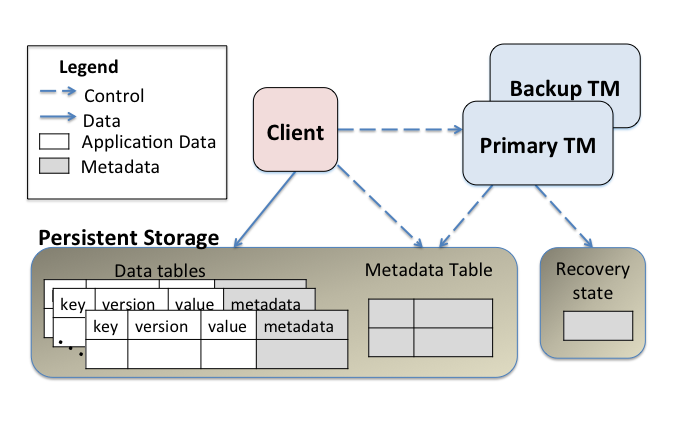
\includegraphics[width = 0.95\columnwidth]{OmidComponents.png}
}
\caption{{\bf \sys\ architecture}. Clients manipulate data that resides in data tables in the underlying multi-versioned persistent data store (for example, HBase) and use the TM in the control path for conflict detection. Only the primary TM is active, and the backup is in hot standby mode. The TM maintains persistent metadata in the data store as well as separately managed recovery state (for example, using Zookeeper).}
\label{fig:Omid_Architecture}
\end{figure}


% MV
\sys\ leverages  \emph{multi-versioning}  in the underlying key-value store in order to allow transactions to read consistent snapshots of changing data as needed for snapshot isolation. The store's API allows users to manipulate versions explicitly. It supports atomic {\em put(key, val, ver)}  and  {\em putIfAbsent(key, val, ver)} operations for updating or inserting a new  item with a specific version, and an atomic {\em get(key, ver)} operation for retrieving the item's value with highest version not exceeding \emph{ver}.
Specifically, when the item associated with an existing key is overwritten, the new version (holding the key, its new value, and a new version number)  is created, while the previous version persists. 
An old version might be required as long as there is some active transaction that had begun before the transaction that overwrote this version has committed. Though this may take a while, overwritten versions eventually become obsolete. 
A cleaning process, (in HBase, implemented as a coprocessor~\cite{hbase-coproc}),
%\footnote{\small{\url{https://blogs.apache.org/hbase/entry/coprocessor_introduction}}}) 
frees up the disk space taken up by obsolete versions. 


% TM  
The transaction control plane is implemented by a centralized transaction manager.
%, backed by persistent storage in the underlying data store. 
The TM has three roles: (i) \emph{version (timestamp) allocation} for each transaction; (ii) \emph{conflict detection} in order to determine which transactions may commit; 
and (iii) \emph{persistent logging of the commits}.
The TM provides high availability via a primary-backup approach--- if the primary TM becomes unresponsive, then the backup becomes the new primary and takes over. 
This design offers durability and high availability; it further facilitates scalability of storage and compute resources separately -- 
metadata storage access scales out on the underlying distributed data store, whereas 
conflict management is done entirely in RAM, and scales up on a shared-memory multi-core server. 

% TM conflict detection
Conflict detection
is lightweight and can be performed at a high throughput -- at least an order of magnitude faster than the transaction 
processing rates the network can sustain.
For example, with 
eight threads, it can handle 
%typical workload at the rate of 
five million transactions per second.
%, with an average of two data items accessed per transaction. 
To reduce the communication cost and RAM footprint of the TM, we use approximate conflict detection, which is 
based on hashes rather than  full keys, and also represents some information in aggregate form. 
Although this may lead to false aborts, the abort rates witnessed both in production and 
in microbenchmarks are negligible.

% We describe the commit protocol and conflict detection mechanism in Section~\ref{sec:protocol}.

% HA
Our high availability solution tolerates ``false'' fail-overs, where a new primary replaces one that is simply slow,
(for example, due to a garbage collection stall), leading to a period with two active primaries.
Synchronization between the two  is based on  shared persistent metadata storage, 
and induces overhead only in rare cases when more than one TM acts as primary.
\sys\ uses time-based leases in order to minimize potential overlap among primaries. 
The implementation employs Apache Zookeeper~\cite{zookeeper}
%\footnote{\small{\url{http://zookeeper.apache.org}.}} 
for lease management and synchronization between primary and backup. 
%This mechanism is described in detail in Section~\ref{sec:ha}.


\section{Related Work}
\label{sec:related}

Distributed transaction processing has been the focus of much interest in recent years. Most academic-oriented papers~\cite{Aguilera2015, Aguilera2007, Balakrishnan2013, Cowling2012, Dragojevic2015, Thomson2012, DBLP:conf/sosp/ZhangSSKP15} build full-stack solutions, 
which include transaction processing as well as a data tier. Some new protocols exploit advanced hardware trends like RDMA and HTM~\cite{Dragojevic2014, Dragojevic2015, Wei2015}. Generally speaking, these solutions do not attempt to maintain separation of concerns between different layers of the software stack, neither in terms of backward compatibility nor in terms of development efforts. They mostly provide strong consistency properties such as serializability.
% or even strict serializability.

On the other hand, production systems such as Google's Spanner~\cite{Spanner2012}, Megastore~\cite{Megastore} and Percolator~\cite{Percolator2010}, 
Yahoo's Omid1~\cite{OmidICDE2014},  Cask's Tephra~\cite{Tephra}, 
and more~\cite{Warp,PattersonENAA12,cockroach}, are inclined towards separating the responsibilities of each layer. These  systems, like the current work, reuse 
an existing persistent highly-available data-tier;
%, which is already deployed and used in production.
for example, Megastore is layered on top of Bigtable~\cite{Chang2008},  Warp~\cite{Warp} uses HyperDex~\cite{Escriva2012},
and CockroachDB~\cite{cockroach} uses RocksDB. 

\sys\ most closely resembles Tephra~\cite{Tephra} and Omid1~\cite{OmidICDE2014}, which also run on top of a distributed key-value store and leverage a centralized TM (sometimes called \emph{oracle}) for timestamp allocation and conflict resolution. 
However, 
Omid1 and Tephra  store all the information about committed and aborted transactions in the TM's RAM, and  proactively duplicate it to every client that begins a transaction (in order to allow the client to determine locally which non-committed data should be excluded from its reads). 
This approach is not scalable, as the information sent to clients can consist of many megabytes. 
\sys\ avoids such bandwidth overhead by storing pertinent information in a metadata table that clients can access as needed.
Our performance measurements in Section~\ref{sec:eval} below show that \sys\ significantly out-performs Omid1, whose design is very close to Tephra's. 
For high availability, Tephra and Omid1 use a write-ahead log, which entails long recovery times for replaying the log; 
\sys, instead, reuses the inherent availability of the underlying key-value store, and  hence recovers quickly from  failures.

Percolator also uses a centralized ``oracle'' for timestamp allocation but  resolves conflicts via two-phase commit, whereby 
clients lock database records rendering them inaccessible to other transactions;
the Percolator paper does not discuss high availability. Other systems like Spanner and CockroachDB allot globally increasing
timestamps using a (somewhat) synchronized clock service. Spanner also uses two-phase commit whereas CockroachDB uses
distributed conflict resolution where read-only transactions can cause concurrent update transactions to abort. In contrast, \sys\ never locks
(or prevents access to) a database record, and never aborts due to conflicts with read-only transactions.

The use cases production systems serve allow them to provide SI~\cite{Percolator2010,OmidICDE2014,Tephra,cockroach}, at least for read-only transactions~\cite{Spanner2012}. It is nevertheless straightforward to 
extend \sys\ to provide serializability, similarly to a serializable extension of Omid1~\cite{YabandehCritique2012} and Spanner~\cite{Spanner2012}; 
it is merely a matter of extending the conflict analysis to cover read-sets~\cite{FeketeTODS2005,Cahill2008}, which may degrade performance. 

A number of other recent efforts avoid the complexity of two-phase commit~\cite{DBLP:conf/sigmod/GrayHOS96} by serializing 
transactions using a global serialization service such as highly-available log~\cite{Balakrishnan2013, eyal2013ordering, Hyder} or totally-ordered multicast~\cite{Camargos07sprint}. \sys\ is unique in utilizing a single transaction manager to resolve conflicts in a scalable way. 




\section{Service Semantics and Interface}
\label{sec:semantics}

\sys\ provides transactional access to a large collection of persistent data items identified by unique keys. 
The service is persistent and highly available, 
whereas its clients are ephemeral, i.e., they are alive only when performing operations and may fail at any time.
We now discuss the semantics and API \sys\ offers.

{\paragraph{Semantics.} 
A \emph{transaction} is a sequence of put and get operations on different objects that ensures the so-called ACID properties:
\emph{atomicity} (all-or-nothing execution), \emph{consistency} (preserving each object's semantics), 
\emph{isolation} (in that concurrent transactions do not see each other's partial updates), and 
\emph{durability} (whereby updates survive crashes).

Different isolation levels can be considered for the third property. \sys\ opts for  snapshot isolation~\cite{DBLP:conf/sigmod/BerensonBGMOO95}, which is provided by popular database technologies such as Oracle, PostgreSQL, and SQL Server. 
Intuitively, SI ensures that the information a transaction retrieves from the database 
does not mix old and new values. For example, if a task updates the values of two stocks, then no other transaction may observe the old value of one of these stocks and the new value of the other. 
%
More precisely, SI enforces a total order on committed transactions according to their commit times so that 

\begin{enumerate}
    \setlength{\itemsep}{0pt}
    \setlength{\parskip}{0pt}
    \setlength{\parsep}{2pt}  
\item
each transaction's get operations see a consistent snapshot of the database reflecting put operations by
 exactly those transactions that committed prior to the transaction's start time; and 
\item
 a transaction commits only if none of the items it updates has been modified since that snapshot.
 \end{enumerate}
Note that under SI,  concurrent transactions conflict only if they  \emph{update} the same item, whereas with 
serializability, a transaction that updates an item conflicts with transactions that \emph{get} that item. Thus, for read-dominated workloads, SI is amenable to implementations (using multi-versioned concurrency control) that 
allow more concurrency than serializable ones, and hence scale better.

\paragraph{API.} 
\sys's client API offers abstractions both for control (\emph{begin, commit}, and \emph{abort}) and for data access (\emph{get} and \emph{put}). Programmers  delineate transactions via the begin and commit APIs: 
the sequence of get and put operations a client invokes between begin and  commit pertains to one transaction.
Following a commit call, the transaction may successfully \emph{commit}, whereby all of its operations take effect;
in case of conflicts, (i.e., when two concurrent transactions attempt to update the same item), the transaction may
\emph{abort}, in which case none of its changes take effect. An abort may also be initiated by the programmer, e.g., 
on encountering an error. Applications typically retry a transaction upon (either type of) abort. 
\sys's API is offered by a client library, which accesses the data directly in the data store, and interacts with the TM only to begin, commit, or abort transactions. 






\section{Transaction Processing}
\label{sec:protocol}


We now explain how \sys's TM manages transactions so as to guarantee  SI semantics. For clarity of the exposition, we defer discussion of the TM's reliability  to the next section; for now, let us assume that this component never fails. 
We describe \sys's data model in Section~\ref{ssec:data-model}, then proceed to describe the client operation in Section~\ref{ssec:client-side} and the TM's operation in Section~\ref{ssec:server-side}.

\subsection{Data and metadata}
\label{ssec:data-model}

% Timestamps
\sys\ employs optimistic concurrency control with commit-time conflict resolution. Intuitively, with SI, a transaction's reads all appear to occur at one logical point in time (namely, when it begins), while its writes appear to execute at a later point--- when it commits. \sys\ therefore associates two timestamps with each transaction: a \emph{read timestamp} $ts_r$ when it begins, and a \emph{commit timestamp} $ts_c$ upon commit. Both timestamps are provided by the TM using a logical clock it maintains. In addition, each transaction has a unique transaction id \emph{txid}, 
for which we use the read timestamp; in order to ensure its uniqueness, the TM increments the clock whenever a transaction begins. 

% Multi-versioning and snapshots 
The data store is multi-versioned. A write operation by a transaction starting at some time $t$ needs to be associated with a version number that exceeds all those written by transactions that committed before time $t$. However, the version order among concurrent transactions that  attempt to update the same key is immaterial, since at least one of these transactions is doomed to abort. To ensure the former, 
we use the writing transaction's \emph{txid}, which exceeds that of all previously committed transactions, as the version number. Multi-versioning is then used in conjunction with the read timestamp to ensure that a transaction's get operations observe a consistent snapshot of the data reflecting all updates by  transactions that committed before the reading transaction began. 

% Atomic commit at the commit table
Since transaction commit needs to be an atomic step, \sys\ tracks the list of committed transactions in a persistent
 {\em Commit Table (CT)}, as shown in Table~\ref{table:data-model}, which in the current implementation is also stored in HBase.
Each entry in the CT maps a committed transaction's \emph{txid} to its respective $ts_c$.
When deciding to commit a transaction, the TM writes the $(txid, ts_c)$ pair to the CT, which makes the transaction durable, and is considered the commit point of the transaction.
%Transactions' put operations write their information (with the $txid$) to the data store whereas 
Gets refer to the CT using the $txid$ in the data record in order to find out if a read value has been committed or not.
In case it has, they use the commit timestamp to decide whether the value appears in their snapshot.

While checking the CT for every read ensures correctness, it imposes  communication costs and  contention on the CT.
To avoid this overhead, \sys\ augments each record in the data store with a {\em commit field (cf)}, indicating whether the data is committed, and if it is, its commit timestamp.
Initially the commit field is \emph{nil}, indicating that the write is \emph{tentative}, i.e., potentially uncommitted.
Following a commit, the transaction updates the commit fields of its written data items with its $ts_c$, and then removes itself from the CT. 
Only then, the transaction is considered complete. 
%(although it has committed earlier).
A background cleanup process helps old (crashed or otherwise slow) committed transactions complete.

Table~\ref{table:data-model} shows an example of a key $k_1$ with two versions, the second of which is tentative.  
%Note that each record consists of four fields \emph{(key, value, version, commit)}.
A transaction that encounters a tentative write during a read still refers to the CT in order to find out whether the value has been committed. In case it has, it helps
complete the transaction that wrote it by copying its $ts_c$ to the commit field. The latter is an optimization that might reduce accesses to the commit table by ensuing transactions.

\begin{table}
\begin{tabular}{|c|c|c|c| c| c | c|}
\multicolumn{4}{c}{Data Table}&  \multicolumn{3}{r}{\hspace{1mm} Commit Table}\\
\cline{1-4} \cline{6-7}
key & value & version & commit & & \emph{txid} & commit \\
 &  & (\emph{txid}) & (cf) & &  &  $ts$  \\
\cline{1-4} \cline{6-7}
$k_1$ & a & {\bf 5} & 7& & {\bf 5} & 7 \\
\cline{6-7}
$k_1$ & b & {\bf 8} & nil \\
\cline{1-4}
\end{tabular}

\caption{{\bf \sys\ data and metadata}. Data is multi-versioned, with the $txid$ as the version number. The \emph{commit field} indicates whether the data is committed, and if so, its commit timestamp. The commit table (CT) maps incomplete committed transaction ids to their respective commit timestamps. Transaction 5 has already committed and updated cf for $k_1$, but has not yet removed itself from CT; transaction 8 is still pending.}
\label{table:data-model}
\end{table}

\subsection{Client-side operation}
\label{ssec:client-side}

\begin{algorithm}[ht!]
\begin{algorithmic}[1]
\begin{small}
\State local variables \emph{txid}, write-set
%\Statex
\Procedure{begin}{}
\State \emph{txid} $\leftarrow$ {\sc tm.begin()}
\State write-set $\leftarrow \emptyset$
\EndProcedure
%\Statex
\Procedure{put}{key, value} 
\State ds.put(key, value, $txid$, nil) \label{l:put}
\State add 64-bit hash of key to write-set
\EndProcedure
%\Statex
\Procedure{get}{key} 
\For{rec $\leftarrow$ ds.get(key, versions down from $ts_r$)} \label{l:get_loop}
   \If{rec.commit$\not=$nil} \Comment not tentative
      \If{rec.commit $< ts_r$}  \State return rec.value  \label{l:get_found} \EndIf
   \Else \Comment tentative
      \State value $\leftarrow$ {\sc GetTentativeValue}(rec, key)
      \If{value $\not=$nil}  
	\State return value
      \EndIf
   \EndIf
\EndFor
\State return nil
\EndProcedure
%\Statex
\Procedure{GetTentativeValue}{rec,key} \label{l:get_tentative}
 \State lookup rec.version in CT
 \If{present} \Comment  committed
       \State update rec.commit \Comment helping 
       \If{rec.commit $< ts_r$}  return rec.value \EndIf
\Else
\Comment re-read version not found in CT \label{l:get_reread}
         \State  rec $ \leftarrow$ ds.get(key, rec.version) 
         \If{rec.commit$\not=$nil $\wedge$ rec.commit $< ts_r$}  
		\State return rec.value \EndIf %\EndIf
\EndIf
\State return nil
\EndProcedure
%\Statex
\Procedure{commit}{}
\State  $ts_c \leftarrow$ {\sc tm.commit}($txid$, write-set)
\ForAll{$key$ in write-set}
	\State rec $\leftarrow$ ds.get(key, $txid$)
	\If{$ts_c = \bot$} \Comment abort
		\State remove rec
	\Else
		\State rec.cf $\leftarrow ts_c$  
	\EndIf
\EndFor
\State remove record with $txid$ from CT
\EndProcedure
\end{small}
\algstore{omid}
\end{algorithmic}
\caption{\sys's client-side code.} 
\label{fig:get-pseudocode}
\end{algorithm} 

% Flow
Transactions proceed optimistically and are validated at commit time. In the course of a transaction, a client's get operations read a  snapshot 
reflecting the data store state  at  
their read timestamp, while put operations write tentative values with $txid$. 
Since SI needs to detect only write-write conflicts, only the transaction's \emph{write-set} is tracked.
%
%The \sys\ transaction flow is depicted in Figure~\ref{fig:flow}, and proceeds as follows:
The  operations, described in pseudocode in Algorithm~\ref{fig:get-pseudocode},   execute as follows:

%\noindent
{\bf Begin.} The client obtains from the TM a read timestamp $ts_r$, 
which also becomes its transaction id ({\em txid}). 
The TM ensures that this timestamp exceeds all the commit timestamps of committed transactions
and precedes all commit timestamps that will be assigned to  committing transactions in the future.

{\bf Put(key,val).} 
The client adds  the tentative record 
%\emph{(key, val, txid, nil)}  
to the data store (line~\ref{l:put}) and tracks the key in its local \emph{write-set}.
 To reduce  memory and communication overheads, we track $64$-bit hashes rather than  full keys. 

{\bf Get(key).} A get 
reads from the data store (via ds.get()) records pertaining to \emph{key} with versions smaller than $ts_r$, latest to earliest
(line \ref{l:get_loop}),
in search of the value written for this key by the latest transaction whose $ts_c$ does not exceed $ts_r$ (i.e., the latest version written by a transaction that committed before the current transaction began).
% Since the version is the writing transaction's  read timestamp ($txid$), it provides a lower bound on the record's commit timestamp. 

If the read value is committed with a commit timestamp lower than $ts_r$, it is returned (line~\ref{l:get_found}).
Upon encountering a tentative record (with cf=\emph{nil}), the algorithm calls {\sc GetTentativeValue} (line~\ref{l:get_tentative}) 
in order to search its $ts_c$ in the CT. 
If this $txid$ was not yet written, % in the CT, 
then it can safely be ignored, since it did not commit. However, 
a subtle race could happen if the transaction has updated the commit timestamp 
in the data store and then removed itself from the CT between the time the record was read and the time when the CT was checked.
In order to discover this race, a record is re-read after its version is not found in the CT (line~\ref{l:get_reread}).
In all cases, the first value encountered in the backward traversal
with a commit timestamp lower than $ts_r$ is returned.

{\bf Commit.} The client requests \emph{commit(txid, write-set)} from the TM.
The TM assigns it a commit timestamp $ts_c$ and checks for conflicts. If there are none, it commits the transaction by writing  $(txid, ts_c)$ to the CT and returns a response. Following a successful commit,
the client writes  $ts_c$ to 
the commit fields of all the data items it wrote to (indicating that they are no longer tentative), and finally 
deletes its record from the CT.
%A client never leaves the data store in an inconsistent state. 
Whether the commit is successful or not 
a background process helps transactions to complete or cleans their uncommitted records from the data store, thereby overcoming client failures.

\subsection{TM operation}
\label{ssec:server-side}

The TM uses an internal (thread-safe) clock to assign read and commit timestamps.
Pseudocode for the TM's begin and commit functions is given in Algorithm~\ref{fig:commit-pseudocode}; both  
operations increment the clock and return its new value. 
Thus, read timestamps are unique and can serve as transaction ids. Begin returns once all transactions with smaller commit timestamps are finalized, 
(i.e., written to the CT or aborted).

Commit involves {compute} and  {I/O} aspects for conflict detection and CT update, resp.
The TM uses a pipelined SEDA architecture~\cite{SEDAPhDThesis} that 
scales each of these stages separately using multiple threads.
Note that the I/O stage also benefits from such parallelism since the 
%underlying data store holding the 
CT can be sharded across multiple storage nodes and yield higher throughput when accessed in parallel.

In order to increase throughput, writes to the commit table are batched. Both begin and commit operations need to wait for batched writes to complete before they can return -- begin waits for all smaller-timestamped transactions to be persisted, while commit waits for the committing transaction.
Thus, batching introduces a tradeoff between I/O efficiency, (i.e., throughput), and begin/commit latency.

The {\sc ConflictDetect}
function checks for conflicts using a hash table in main memory.  (The TM's compute aspect is scaled by running multiple instances of this function for different transactions, accessing the same table in separate threads.)
For the sake of conflict detection, every entry in the write-set is considered a \emph{key}, 
(though in practice it is a $64$-bit hash of the appropriate key). 
Each \emph{bucket} in the hash table holds an array of pairs, each consisting of a key hashed to this bucket 
and  the $ts_c$  of the transaction that last wrote to this key.

{\sc ConflictDetect} needs to (i) validate that none of the keys in the write-set have versions larger than $txid$ in the table, and (ii) if validation is successful, update the  table entries pertaining to the write-set to the transaction's newly assigned $ts_c$. However, this needs to be done atomically, so two transactions committing in parallel won't miss each other's updates. 
Since holding a lock on the entire table 
for the duration of the conflict detection procedure would severely limit concurrency, we instead limit the granularity of atomicity to a single bucket: for each key in the write-set, we lock the corresponding bucket (line~\ref{l:lock}), 
check for conflicts in that bucket
(line~\ref{l:conflict}), and if none are found, optimistically add the key with the new $ts_c$ to the bucket (lines~\ref{l:update-start}--\ref{l:update-end}). The latter might prove redundant in case the transaction ends up aborting due to a conflict it discovers later. However, since our abort rates are low, such spurious additions rarely induce additional aborts.

\begin{algorithm}[htb]
\begin{algorithmic}[1]
\algrestore{omid}
\begin{small}
\Procedure{begin}{}
\State $txid$ = Clock.FetchAndIncrement()
\State wait until there are no pending commit operations 
\State \hspace{18pt} with $ts_c < txid$
\State return $txid$
\EndProcedure
\Statex
\Procedure{commit}{$txid$, write-set}
\State $ts_c \leftarrow$ Clock.FetchAndIncrement()
\If{ConflictDetect($txid$, write-set) = {\sc commit}} 
 \State UpdateCT($txid, ts_c$) \Comment proceed to I/O stage
 \State return $ts_c$
 \Else
 \State return {\sc abort}
\EndIf
\EndProcedure
\Statex
\Procedure{ConflictDetect}{$txid$,write-set}
\ForAll{key $\in$ write-set} 
  \State b $\leftarrow$ key's bucket
  \State lock b  \label{l:lock}
  \State small $\leftarrow$ entry with smallest $ts$ in b
  \If{$\exists$ (key, t) $\in $ b s.t.\ $t > txid$ } \Comment conflict  \label{l:conflict}
    \State unlock b; return {\sc abort}
  \EndIf
  \Statex 
  \Comment no conflict on key found -- update hash table 
  \If{$\exists$ (key, t) $\in $ b s.t.\ $t < txid$ }  \label{l:update-start}
    \State overwrite (key, t) with (key, $ts_c$)
    \ElsIf{$\exists$ empty slot $s \in $ b }
    \State write (key, $ts_c$) to $s$
    \ElsIf{ small.$t \le txid$ } 
	      \State overwrite small with (key, $ts_c$)  \label{l:update-end}
     \Else  \Comment possible conflict  \label{l:possible-conflict}
   \State unlock b; return {\sc abort}
  \EndIf  
\State unlock b
\EndFor
\State return {\sc commit}
\EndProcedure
\end{small}
\algstore{omid}
\end{algorithmic}
\caption{TM functions.} 
\label{fig:commit-pseudocode}
\end{algorithm} 

A second challenge is to limit the table size and garbage-collect information pertaining to old commits. Since a transaction need only check for conflicts with transactions whose $ts_c$ exceeds its $txid$, it is safe to remove all entries that have smaller commit times  than the $txid$ of the oldest active transaction. Unfortunately, this observation does not give rise to a feasible garbage collection rule:
though transactions usually last few tens of milliseconds, there is no upper bound on  a transaction's life span, and no way to know whether a given outstanding transaction will ever attempt to commit or has failed. 
Instead, we use the much simpler policy of restricting the number of entries in a bucket. Each bucket holds a fixed array of the most recent $(key, ts_c)$ pairs. In order to account for potential conflicts with older transactions, a transaction also aborts in case the minimal $ts_c$ in the bucket exceeds its $txid$ (line \ref{l:possible-conflict}). 
In other words, a transaction expects to find, in every bucket it checks, at least one commit timestamp older than its start time or one empty slot, 
and if it does not, it aborts.

The size of the hash table is chosen so as to reduce the probability for spurious aborts, which is the probability of  all keys in a given bucket being replaced during a transaction's life span. 
If the throughput is $T$ transactional updates per second, a bucket in a table with $e$ entries will overflow after $e/T$ seconds on average. For example, if $10$ million keys are updated per second, 
a bucket in a one-million-entry table will overflow only after 100ms on average, which is much longer than most transactions. We further discuss the impact of the table size in Section~\ref{sec:eval}. 

\paragraph{Garbage collection.} A dedicated background procedure ({\em co-processor}) cleans up old versions. To this end, the TM maintains 
a \emph{low water mark}, which is used in two ways: (1) the co-processor scans data store entries, and keeps, for each key,
the biggest version that is smaller than the low water mark along with all later versions. Lower versions are removed.
(2) When a transaction attempts to commit, if its $txid$ is smaller than the low water mark, it aborts because the co-processor may 
have removed versions that ought to have been included in its snapshot. 
The TM attempts to increase the low water mark when the probability of such aborts is small.

\remove{
For example, at a throughput of $10$ million transactional updates per second, buckets in a table with one million entries, (for example, 62500 buckets of size 16),  will overflow only after 100ms on average, which is much longer than most transactions. Since both keys and timestamps are $8$ bytes long, the table size in this case is merely $16$MB, which easily fits in L2 caches in modern servers.  
}



\section{High Availability}
\label{sec:ha}

%%%%

Very-high-end \sys-powered applications are expected to work around the clock, with a mean-time-to-recover of just a few seconds. \sys\ therefore needs to provide \emph{high availability (HA)}. 
Given that the underlying  data store is already highly available
and that client failures are tolerated by \sys's basic transaction processing protocol, 
\sys's HA solution only needs to address TM failures.
This is achieved via the primary-backup paradigm: during normal operation, a single \emph{primary} TM handles client requests, while a \emph{backup} TM runs in hot standby mode.
Upon detecting the primary's failure, the backup performs a \emph{failover} and becomes the new primary. 

The backup TM may falsely suspect that the primary has failed.
The resulting potential simultaneous operation of more than one TM creates challenges, which we discuss in 
Section~\ref{ssec:failover}. We address these in Section~\ref{ssec:basic} 
by adding synchronization to the transaction commit step. While such synchronization ensures correctness, it also introduces substantial overhead. We then optimize the solution in Section~\ref{ssec:opt}
to forgo synchronization during normal (failure-free) operation.

Our approach thus resembles 
many popular protocols, such as Multi-Paxos~\cite{Lamport:1998:PP:279227.279229} and its variants, which expedite normal mode operation as long as an agreed leader remains operational and unsuspected. However, by relying on shared persistent state in the underlying highly available data store, we obtain a simpler solution, eliminating the need to synchronize with a quorum in normal mode or to realign state during recovery.

%The latter is the actual implementation in \sys.  

\subsection{Failover and concurrent TMs} 
\label{ssec:failover}

The backup TM constantly monitors the primary's liveness.
Failure detection is timeout-based, namely, if the primary TM does not re-assert its existence within a configured period, it is deemed failed, and the backup starts acting as primary.  
Note that the primary and backup run independently on different machines, and the time it takes the primary to inform the backup that it is alive can be unpredictable due to network failures and processing delays, (e.g., garbage-collection stalls or long I/O operations). But in order to provide fast recovery, it is undesirable to set the timeout conservatively so as to ensure that a live primary is never detected as faulty.

We therefore have to account for the case that the backup performs failover and takes over the service while the primary is operational. 
Though such simultaneous operation of the two TMs is a necessary evil if one wants to ensure high availability, our design strives to reduce such overlap to a minimum. To this end, the primary TM actively checks if a backup has replaced it, and if so, ``commits suicide'', i.e., halts. However, it is still possible to have a (short) window between the failover and the primary's discovery of the existence of a new primary when two primary TMs are active. 

When a TM fails, all the transactions that began with it and did not commit (i.e., were not logged in the CT) are deemed aborted. 
%To prevent new transactions from seeing partial updates of transactions handled by the old TM, 
%The new TM needs to pick a starting logical clock time that exceeds all commit timestamps of transactions 
%that might still be committed by the old TM. 
However, this clear separation is challenged by the potential simultaneous existence of two TMs. For example, if the TM fails while a write it issued to the CT is still pending, the new TM may begin handling new transactions before the pending write takes effect. Thus, 
an old transaction may end up committing after the new TM has begun handling new ones. Unless handled carefully, this can cause a new transaction to see partial updates of old ones, as illustrated in Figure~\ref{fig:2TMs}.
To avoid this, we must ensure that once a new transaction obtains a read timestamp, the status of all transactions with smaller commit timestamps does not change.

A straightforward way to address the above challenge is via mutual exclusion, i.e., making sure that at most one TM commits operations at a time. However, this solution would entail synchronization upon each commit, not only at failover times, which would adversely affect performance. We therefore forgo this option.

\begin{figure}[t]
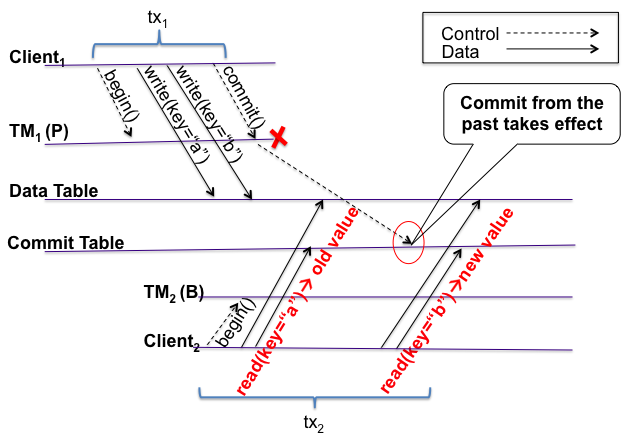
\includegraphics[width=\columnwidth]{omid_ha1.png}
\caption{{\bf The challenge with two concurrent TMs.} An old transaction, $tx_1$, commits while a new one $tx_2$ is processed, causing $tx_2$ to see an inconsistent snapshot. }
\label{fig:2TMs}
\end{figure}

\subsection{Basic HA algorithm}
\label{ssec:basic}  

Upon failover from $TM_1$ (the old primary) to $TM_2$ (the new one), we strive to ensure the following  properties:
\begin{description}
\item[P1] all timestamps assigned by $TM_2$ exceed all those assigned by $TM_1$; 
\item[P2] after a transaction $tx_2$ with read timestamp $ts2_r$ begins, no transaction $tx_1$ that will end up with a commit timestamp $ts1_c < ts2_r$ can update any additional data items (though it may still commit); and 
\item[P3] when a transaction reads a tentative update, 
it can determine whether this update will be committed with a timestamp smaller than its read timestamp or not.
\end{description}

Properties P1--P3 are sufficient for SI: P1 implies that commit timestamps continue to be totally ordered by commit time, P2 ensures that a transaction encounters every update that must be included in its snapshot, and P3 stipulates that the transaction can determine whether to return any read value.

To ensure the first two properties, the TMs publish the read timestamps they allot as part of initiating a transaction in a persistent shared object,   \emph{maxTS}. %(our implementation stores it in Apache Zookeeper~\cite{zookeeper}).
Before committing, the TM checks maxTS. If it finds a timestamp greater than its last committed one, it deduces that a new TM is active, aborts the transaction attempting to commit, and halts. 

In Figure~\ref{fig:2TMs} we saw  a scenario where the third property, P3, is violated--- when $tx_2$ reads key $a$ it cannot tell that $tx_1$, which wrote it, will end up committing with a smaller $ts1_c$ than $ts2_r$. 
This leads to an inconsistent snapshot at $tx_2$, as it sees the value of key $b$ written by $tx_1$.

To enforce P3, $tx_2$ cannot wait for $TM_1$, because the latter might have failed. Instead, we have $tx_2$ proactively abort $tx_1$, as illustrated in Figure~\ref{fig:invalidate}. 
%
More generally, when a read encounters a tentative update whose $txid$ is not present in the CT, it forces 
the transaction that wrote it to abort. We call this {\em invalidation}, and extend the CT's schema to include an \emph{invalid} field to this end.
Invalidation is performed via an atomic 
put-if-absent (supported by HBase's {\em checkAndMutate\/} API)
to the CT, which adds a record marking that $tx_1$ has  
``invalid'' status.  
The use of an atomic put-if-absent achieves \emph{consensus} regarding the state of the transaction.

Commits, in turn, read the CT after adding the commit record in order to check whether an invalidation record also exists, and if so, halt without returning a commit response to the client.  
In addition, every read of a tentative update checks its invalid field in the CT, and ignores the commit record if the transaction has been  invalidated.

\begin{figure}[t]
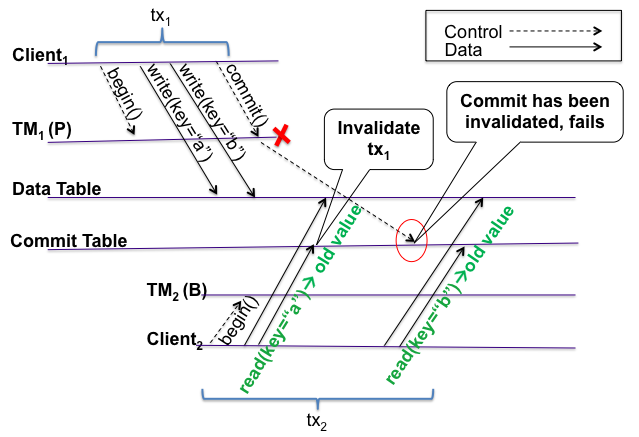
\includegraphics[width=\columnwidth]{omid_ha2.png}
\caption{{\bf Addressing the challenge of two concurrent TMs.} The old transaction is invalidated by the new one and therefore cannot commit.}
\label{fig:invalidate}
\end{figure}

While this solution satisfies the three required properties, it also induces a large number of synchronization steps:
(i) writing allotted read timestamps to maxTS to ensure P1; (ii) checking maxTS at commit time to ensure P2; and (iii)  
%using put-if-absent to invalidate a transaction in the shared CT every time a tentative update is encountered and 
checking  the CT for invalidation at the end of every commit to ensure P3. 
The next section presents an optimization that reduces the cost of synchronization.

\subsection{Synchronization-free normal operation}
\label{ssec:opt}

In order to eliminate the synchronization overhead most of the time, \sys's HA solution uses two mechanisms. 
First, to reduce the overheads  (i) and (ii) associated with timestamp synchronization, it 
allocates timestamp ranges in large chunks, called \emph{epochs}. 
That is, instead of incrementing maxTS by one timestamp at a time, the TM increments it by a certain \emph{range}, 
and is then free to allot timestamps in this range without further synchronization.
Second, to reduce  cost (iii) of checking for invalidations, 
it uses locally-checkable \emph{leases}, which are essentially locks that live for a limited time. As with locks, at most one TM may hold the lease at a given time (this requires the TMs' clocks to advance roughly at the same rate). 
\sys\ manages epochs and leases as shared objects in Zookeeper, and accesses them infrequently. 

Algorithm~\ref{alg:ha} summarizes the changes to support HA. On the TM side, 
{\sc CheckRenew} is called at the start of every commit and begin. 
It first  renews the lease every $\delta$ time, for some parameter $\delta$ (lines~\ref{l:lease-start}--\ref{l:lease-end}).
This parameter defines the tradeoff between synchronization frequency and recovery time:
the system can remain unavailable for up to $\delta$ time following a TM failure.
%
Since clocks may be loosely synchronized, \sys\ defines a {\em guard period\/} of $\delta' < \delta$, 
so that the lease must be renewed at least $\delta'$ time before it expires. 
%We assume the clock skew  between the TMs is smaller than this guard. 
The production default for $\delta'$ is $\delta/4$.
The primary TM fails itself (halts) if it cannot renew the lease prior to that time. 
From the clients' perspective, this is equivalent to a TM crash (line~\ref{l:lease-end}).
Second, {\sc CheckRenew} allocates a new epoch if needed (lines~\ref{l:epoch-start}--\ref{l:epoch-end}).

The backup (not shown in pseudocode) regularly checks the shared lease, and if it finds that it has expired, it immediately sets its clock to exceed maxTS,  
allocates a new epoch for itself (by increasing maxTS), and begins serving requests, \emph{without any special recovery procedure}.
Since the epoch claimed by a new TM always exceeds the one owned by the old one, Property P1 holds. 

Property P2 is enforced by having the TM (locally) check that its lease is valid before committing a transaction
(lines~\ref{l:lease-start}--\ref{l:lease-end}). 
Since at most one TM can hold the lease at a given time, and since the commit is initiated after all writes to items that are part of the transaction complete, Property P2  holds.

Nevertheless, the lease does not ensure Property P3, since the lease may expire while the commit record is in flight,
as in the scenario of Figures~\ref{fig:2TMs} and~\ref{fig:invalidate}. 
To this end, we use the invalidation mechanism described above. However, we limit its scope as follows: 
(1) A commit needs to check whether the transaction has been invalidated only if the TM's lease has expired.
This is done in the {\sc TMCheckInvalidate} function.
(2) A read needs to invalidate a transaction only if it pertains to an earlier epoch of a different TM. 
We extend client's {\sc GetTentativeValue} function to perform such invalidation 
in Algorithm~\ref{alg:ha} lines~\ref{l:invalidate-present},~\ref{l:invalidate-start}--\ref{l:invalidate-end}.
Note that a transaction reading a tentative update still checks its validity status regardless of the epoch, in order to avoid ``helping'' invalidated transactions complete their tentative updates. 
% Note that as long as a single TM is operational, \sys\  runs synchronization-free.





\begin{algorithm}[tb]
\begin{algorithmic}[1]
\algrestore{omid}
\begin{small}
\Procedure{CheckRenew}{} \\
 \Comment called by the TM at start of {\sc Begin} and {\sc Commit} 
\If{lease $<$ now + $\delta'$} \label{l:lease-start}
 \State renew lease for $\delta$ time \Comment atomic operation
 \If{failed} halt \EndIf 
\EndIf  \label{l:lease-end}
\If{Clock $=$ epoch}  \label{l:epoch-start}
\State epoch $\leftarrow$ Clock +  range
\State extend maxTS  from Clock  to epoch 
\If{failed} halt \EndIf 
\EndIf  \label{l:epoch-end}
\EndProcedure
%
\Statex
\Procedure{TMCheckInvalidate}{txid} \\
 \Comment called by the TM before {\sc Commit} returns
\If{lease $<$ now + $\delta'$}
 \If{$txid$ invalid in CT} halt \EndIf 
\EndIf
\EndProcedure
\Statex
%
\Procedure{GetTentativeValue(rec)}{} \\
\Comment replaces same function from Algorithm~\ref{fig:get-pseudocode}
 \State lookup rec.version in CT
 \If{present}
      \If{invalidated} return nil \EndIf 	\label{l:invalidate-present}
       \State update rec.commit \Comment helping
       \If{rec.commit $< ts_r$}  return rec.value \EndIf
\Else
\Comment new code -- check if need to invalidate
\If{rec.version $\in$ old epoch by an old TM} \label{l:invalidate-start}
 \State invalidate $t$ in CT \Comment  try to invalidate
 \If{failed}
	\State lookup rec.version in CT
	\If{invalidated} return nil \EndIf
       \State update rec.commit \Comment helping
       \If{rec.commit $< ts_r$}   \State return rec.value \EndIf
\Else \Comment invalidated
	\State return nil
\EndIf \label{l:invalidate-end}
\Else \Comment original code -- no invalidation
         \State  rec $ \leftarrow$ ds.get(\emph{key}, rec.version)
         \If{rec.commit$\not=$nil $\wedge$ rec.commit $< ts_r$}
		\State return rec.value \EndIf %\EndIf
\EndIf
\EndIf
\State return nil
\EndProcedure
\end{small}
\end{algorithmic}
\caption{\sys's HA algorithm.}
\label{alg:ha}
\end{algorithm}

% {\bf Client failover. }
Finally ,we note that on TM failover, some clients may still
 be communicating with the old TM. While the old TM may
end up committing some of their requests, a problem arises
if the client times out on the old TM before getting the
commit response, since the client might unnecessarily retry a committed transaction. 
To avoid this problem, a client that times out on its TM checks the CT for the status of its transaction
before connecting to a new TM. If the status is still undetermined, the client tries to invalidate the  CT entry, thus either forcing the
transaction to abort or learning that it was committed (in case the invalidation fails). 


\section{Evaluation}
\label{sec:eval}

\sys's implementation complements Apache HBase with transaction processing. 
It exploits HBase to store both  application data and the CT metadata. 
HBase, the TMs, and Zookeeper are all deployed on separate dedicated machines.

In large-scale deployments, HBase tables are  sharded (partitioned) into multiple \emph{regions}.
Each region is managed by a \emph{region server}; one server may serve multiple regions. HBase 
is deployed on top of Hadoop Distributed Filesystem (HDFS), which provides the basic abstraction 
of scalable and reliable storage. HDFS is replicated 3-fold in all the settings described below. 

Section~\ref{sec:prod} presents performance statistics obtained in \sys's 
production deployment, focusing on the end-to-end application-level overhead introduced 
by transaction processing. Section~\ref{sec:synthetic} further zooms in on the TM scalability
under very high loads.
%, via multiple benchmarks. 
%Since the transactions' access to application data is independent of \sys's design, 
%we focus the remaining evaluation, in Section~\ref{sec:thpt}, on benchmarking the TM.

\subsection{End-to-end performance in production}
\label{sec:prod}

We present statistics of \sys's use in a production deployment of Sieve -- Yahoo's
content management system. 
Sieve digests streams of documents from multiple sources, processes them, and indexes 
the results for use in search and personalization applications. Each document 
traverses a pipeline of  tasks, either independently or as part of a mini-batch. 
A task is an  ACID processing unit, framed as a transaction. It typically reads 
one or more data items generated by  preceding tasks, performs some computation, 
and writes one or more artifacts back. 

Sieve scales across task pipelines that serve multiple products,  performing tens of thousands 
of tasks per second on multi-petabyte storage. All  
are powered by a single \sys\ service, with the CT sharded across $10$ regions
managed by $5$ region servers.  
Sieve is throughput-oriented, and favors  scalability over transaction latency. 

\comment{
Table~\ref{table:workload} summarizes the compute and I/O footprint of selected Sieve tasks
within a particular Sieve instance that processes web content, performing tens of thousands 
of tasks per second on multi-petabyte storage. 

\begin{table}[htb]
\centering
\begin{tabular}{| l | l | l |}
\hline
Task	 &  Compute   & \# KV-store \\
         &  time (avg) & accesses (avg)\\
\hline
Document inversion		& 650ms	 & 13 \\
Duplicate detection		& 1.4ms     & 8	\\
Out-link processing		& 35ms      & 3	\\
In-link processing		& 150ms	 & 6	\\
Streaming to runtime		& 2050ms  & 5	\\
\hline
\end{tabular}
\caption{{\bf Production workload.} Task characteristics in a production Sieve deployment powered by \sys.}
\label{table:workload}
\end{table}
}

\begin{figure}[htb]
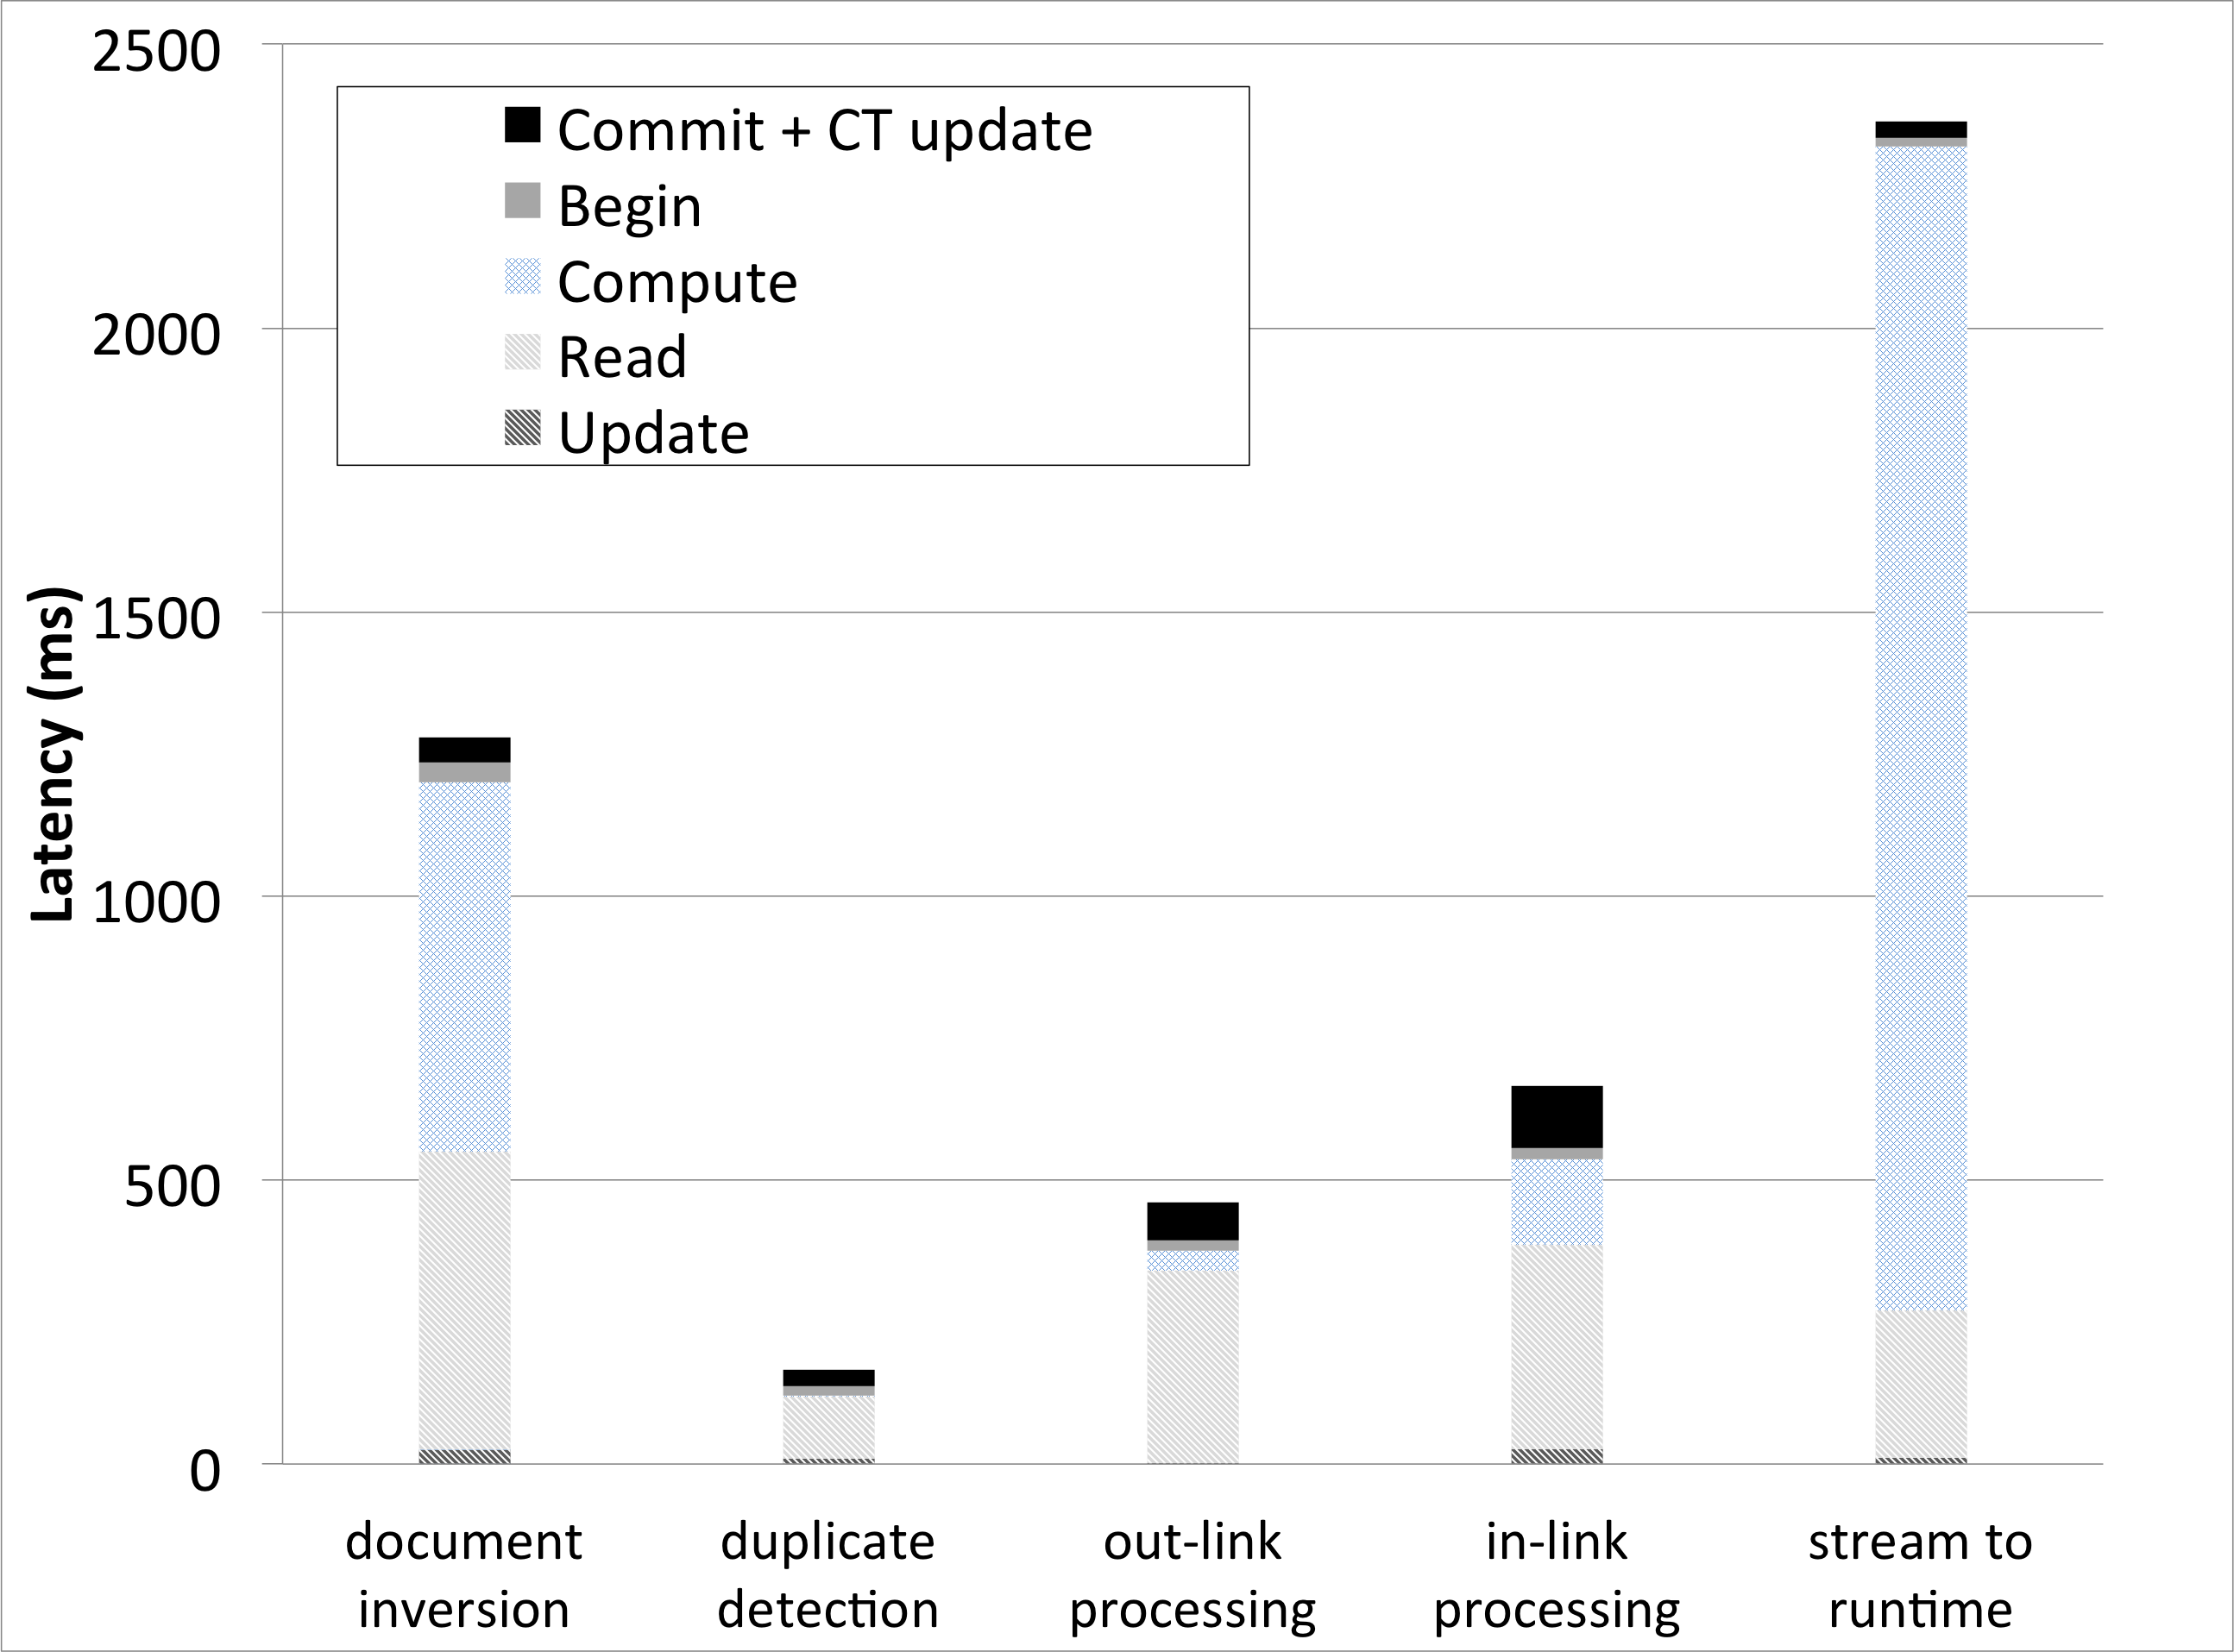
\includegraphics[width=\figw]{Latency-Sieve.png}
\caption{{\bf Transaction latency breakdown in production deployment of \sys\ in Sieve.} The top two components represent 
transaction management overhead.
}
\label{fig:sieve_latency}
\end{figure}

Figure~\ref{fig:sieve_latency} presents statistics gathered for five selected Sieve tasks. 
For each task, we present its average latency broken down to components --
HBase access (two bottom components in each bar), compute time, and the TM's begin and commit  (top two components). 
In this deployment, \sys\ updates the commit fields synchronously upon commit, that is, commit returns only 
after the commit fields of the transaction's write-set have been updated. 
%(the additional latency is reflected in the top component in each bar). 
\remove{
This approach prevents contention on data items produced 
by some task and immediately consumed by the ensuing  task in the pipeline. 
}
Note that since a begin request waits for all transactions with smaller $txids$ to commit, its processing
latency is similar to that of a commit operation, minus the time commit takes to update the commit fields. 


We see that for tasks that perform significant processing and I/O,  like 
document inversion and streaming to index, 
\sys's latency overhead (for processing begin and commit) is negligible --  $2$--$6\%$ of the total transaction duration. 
In very short tasks such as duplicate detection and out-link processing, \sys\ accounts for up to roughly one third of the transaction latency.
%In more latency-sensitive applications, the latency can be further shortened by deferring the commit field updates to execute asynchronously.


The transaction abort rates observed in Sieve are negligible (around $0.002\%$). 
They stem from either transient HBase outages or 
write-write conflicts, e.g., concurrent in-link updates of extremely popular web pages.  

\subsection{TM microbenchmarks}
\label{sec:synthetic}

We now focus on TM performance. 
To this end, our microbenchmarks  invoke only the TM's begin and commit APIs, and do not access actual data.
We run both the TM and HBase (holding the CT) on industry-standard 8-core 
Intel Xeon E5620 servers with 24GB RAM and 1TB magnetic drive. The interconnects  are 1Gbps Ethernet.


We generate workloads in which transaction write-set sizes are distributed Zipf, i.e., follow a power-law ($Pr[X \geq x] = x^{-\alpha}$) 
with exponent values of $\alpha=1.2$, $\alpha=1.6$, and $\alpha=2$ (the smaller the heavier-tailed), cut-off at $256$ keys.
Each transaction's latency, (i.e., the time we wait after invoking its begin and before invoking its commit), is set to $5$ms per write. 
Note that read-sets are not sent to the TM and hence their size is immaterial.

We note that key selection affects \emph{real} conflicts: if the written keys are drawn from a heavy-tailed distribution, then two concurrent 
transactions are likely to update the same key, necessitating one of them to abort. Since this is an artifact of the workload, which is unaffected
by our system design, we attempt to minimize this phenomenon in our experiments. We therefore uniformly sample 64-bit integers
for the key hashes. Recall that our experience in production shows that real conflicts are indeed rare.


We begin by evaluating scalability, which is our principal design goal.
The TM throughput is constrained by two distinct resources -- the storage access required for persisting commits in the CT, and
the compute resources used for conflict detection.
These resources scale independently: the former, evaluated in Section~\ref{ssec:ct-scale}, scales out across multiple HBase region servers, 
whereas the latter scales up on multi-core hardware, and is studied in Section~\ref{ssec:mc-scale}.
Section~\ref{ssec:latency} then evaluates the throughput-latency tradeoff that \sys\ exhibits when using a single region server.
Finally, in Section~\ref{sec:ha-eval}, we exercise \sys's high-availability mechanism. 

\subsubsection{Commit table scalability} 
\label{ssec:ct-scale}

\begin{figure}
\centerline{
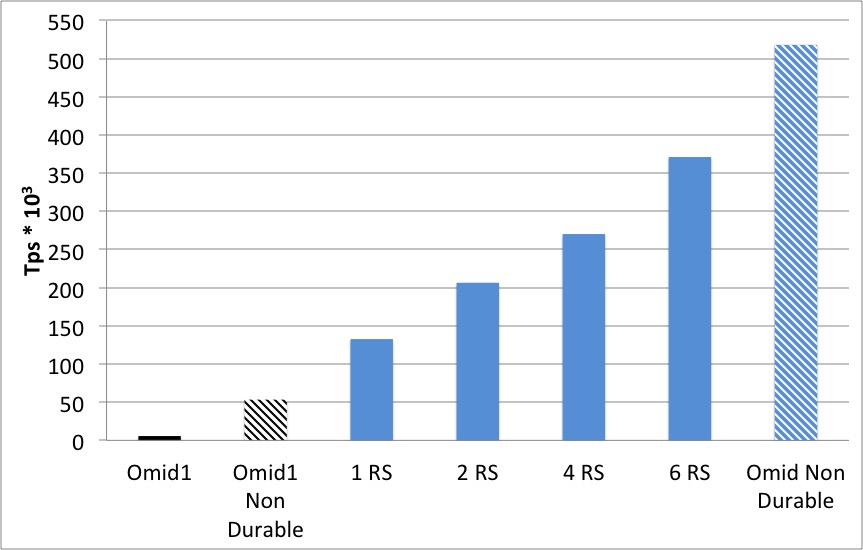
\includegraphics[width=\figw]{CT+Omid1.png}
}
\caption{{\bf Scalability of \sys's CT updates with the number of HBase region servers, and comparison with Omid1.} Non-durable versions do not persist transactions and thus provide upper bounds on throughput under perfect storage scaling. 
%\sys\ uses $4$ writer threads and 2K transaction batches. 
}
\label{fig:ct_thpt}
\end{figure}


Since the commit records are fixed-length (two 64-bit integers), the CT performance does not depend on transaction sizes, and 
so we experiment only with $\alpha=1.6$.
Recall that in order to optimize throughput, the TM batches writes to the CT and issues multiple batches in parallel. 
Experimentally, we found that the optimal number of concurrent CT writer threads is $4$, and  
the batch size that yields the best throughput is 2K transactions per writer. 

Figure~\ref{fig:ct_thpt} depicts \sys's commit rate as function of the number of HBase region servers,
which scales to almost 400K tps.
It further compares \sys's throughput to that of  Omid1~\cite{OmidICDE2014}, which, 
similarly to \sys, runs atop HBase, and uses a centralized TM. 
%and is configured the same way as \sys.  
% with 4 writer threads at the TM side and 6 region servers at the HBase side. 
It is worth noting that even in the single-server configuration, \sys\ outperforms
Omid1  by more than 25x. This happens because upon each begin request, Omid1 sends to the client a large amount 
of information (equivalent to the combination of \sys's CT and the in-memory conflict detection table). 
%Under the studied transaction rates, 
This saturates the CPU and network resources. 

The ``non-durable'' bars -- leftmost and second from the right -- represent experiments where commits are not persisted 
to stable storage. In \sys\ this means forgoing the write to the CT, whereas in Omid1 it means disabling the write to BookKeeper
in which the system stores its commit log.  
These results provide upper bounds on the throughput that can be obtained with perfect storage scaling in both systems. 
\sys\ peaks at 518K transactions per second, whereas Omid1 peaks at 50K. 


\subsubsection{Conflict detection scalability} 
\label{ssec:mc-scale}



\begin{figure*}[tb]
\begin{subfigure}{\columnwidth}
\centerline{     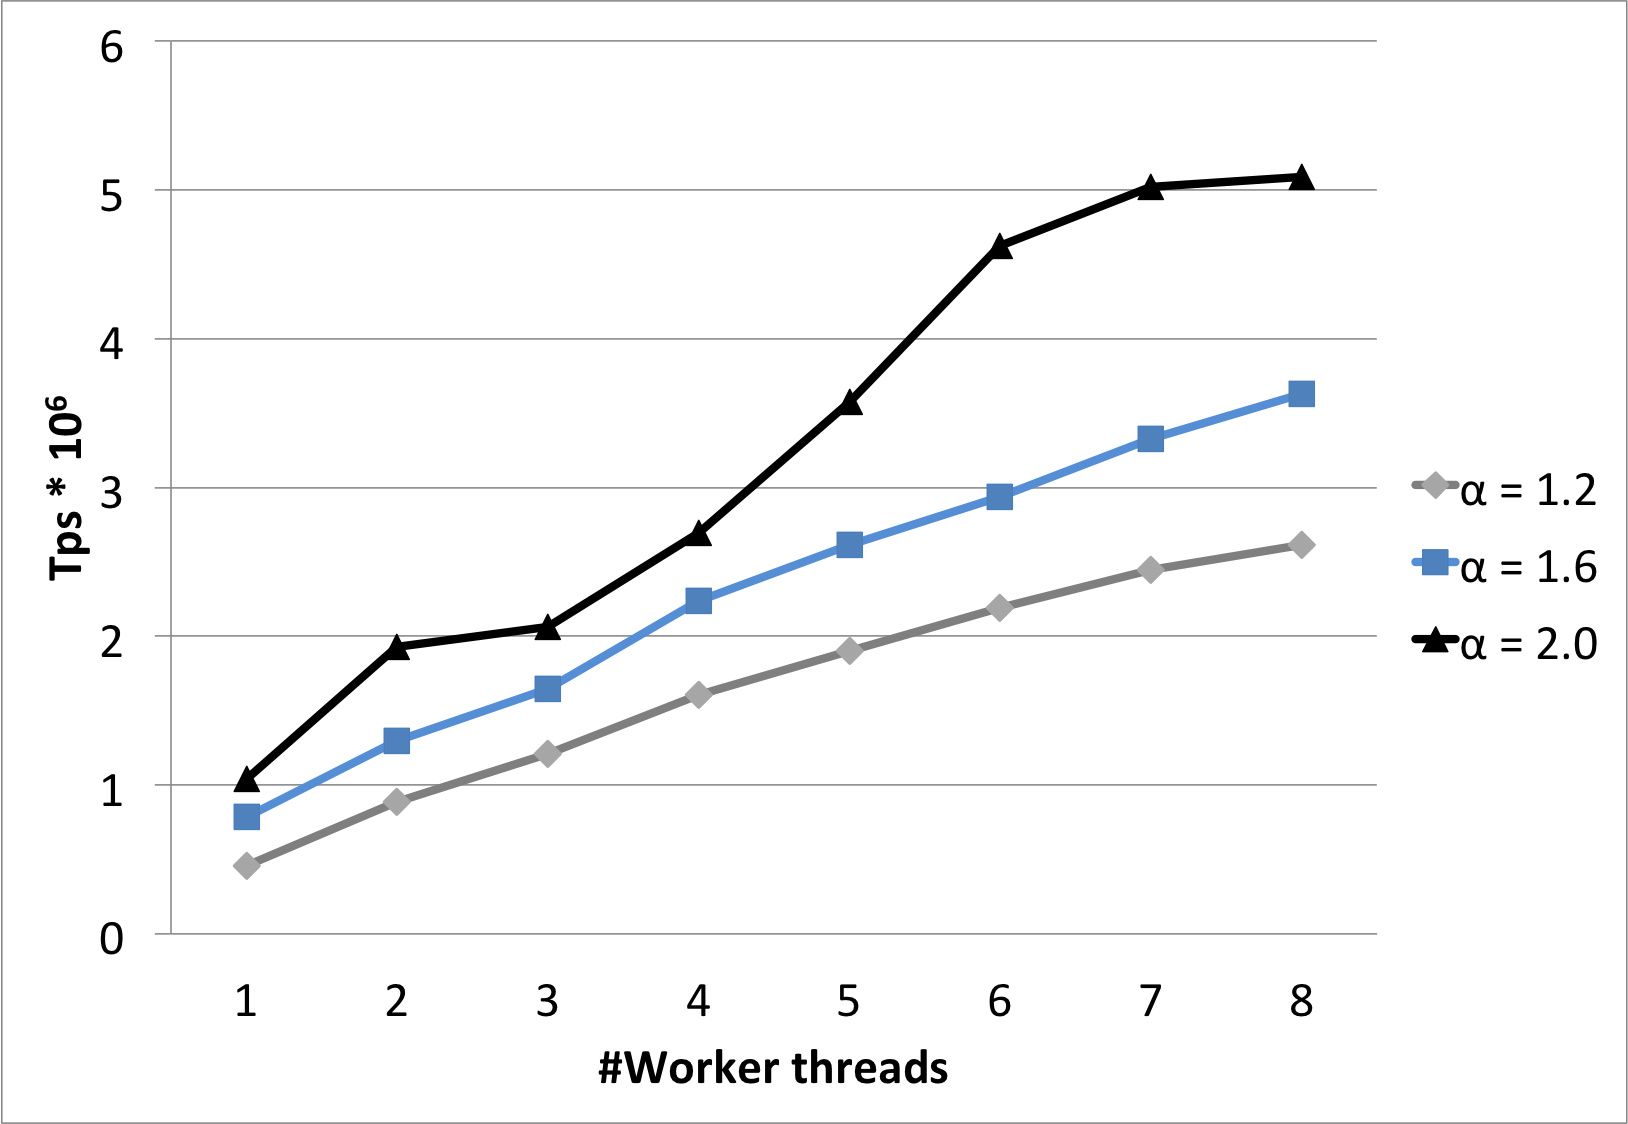
\includegraphics[width=\columnwidth, height=5.25cm]{CDPerf.png} }
	\hspace{0.25cm}
    \caption{Conflict detection scalability}
    \label{fig:1}
  \end{subfigure}
\hspace{\columnsep}
\begin{subfigure}{\columnwidth}
\centerline{      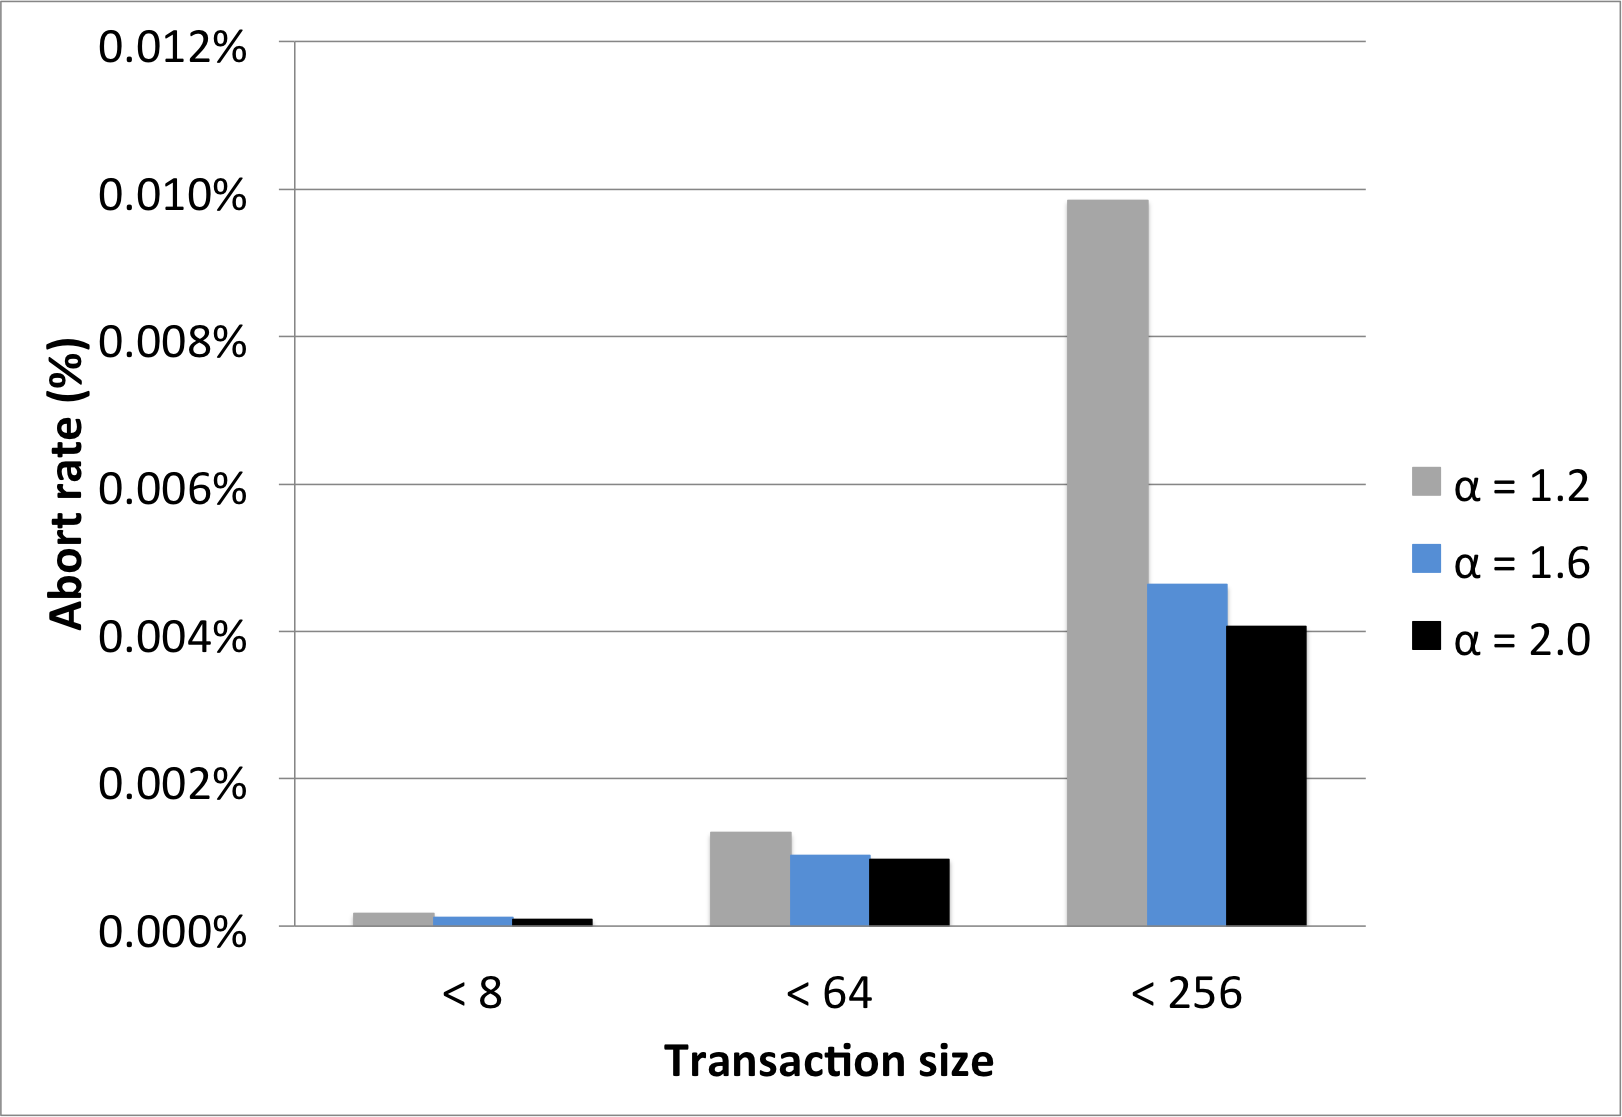
\includegraphics[width=\columnwidth, height=5.25cm]{CDAbort.png} }
	\hspace{0.25cm}
    \caption{Conflict detection false abort rate}
    \label{fig:2}
  \end{subfigure}
\caption{{\bf Conflict detection scalability and false abort rate.} Transaction write-set sizes are distributed power-law ($Pr[X \geq x] = x^{-\alpha}$) 
with exponent values of $\alpha=1.2$, $\alpha=1.6$, and $\alpha=2$ (the smaller the 
heavier-tailed); the key hashes are $6$4-bit integers, uniformly sampled to avoid real conflicts whp; transaction latency is $5$ms per write.}
% 2 plots side by side
\label{fig:cd_perf}
\end{figure*}

In the experiment reported  above, the conflict detection algorithm is evaluated as part of the system.
There, the commit table I/O is the bottleneck, and the conflict detection process can keep up with the pace
of four I/O threads even when running sequentially, i.e., in a single thread. 

We next focus on scale-up of this component running by itself using $1$ to $8$ threads, in order to study its potential scalability in even larger configurations.
The experiment employs a conflict table of 128M 64-bit integers (1G total size). The bucket size is $32$ integers, i.e., the table is 4M buckets big.  

\remove{
When testing the conflict detection component, transaction size is of essence: long transactions are more likely than short ones to
incur spurious aborts due to turnover in hash  buckets. 
We consider three power-law exponent values -- $\alpha=1.2$, $\alpha=1.6$, and $\alpha=2$.
}

Figure~\ref{fig:cd_perf}(a) illustrates the processing rate.
As expected processing shorter transactions (a bigger  $\alpha$) is faster.
%for the three values of $\alpha$. The latency of processing a single commit request is proportional to the transaction size, 
% therefore the throughput is larger for a bigger  $\alpha$ (lighter tail). 
The rate scales to 2.6M transactions per second for $\alpha=1.2$, and to 5M for 
$\alpha=2$. Note that exercising such high throughput in a complete system would require an 
order of magnitude faster network to sustain the request/response packet rate.    
Clearly the TM's compute aspect is far from being a bottleneck.

% Recall that the CD is an imperfect filter with no false negatives. 
Finally, we analyze the false abort rate. (The uniform sampling of key hashes and relatively 
short transaction latencies render real collisions unlikely, hence all aborts 
are deemed false). The overall abort rate is negligibly small. In 
Figure~\ref{fig:cd_perf}(b) we  zoom-in
 on  transactions clustered into three buckets: shorter than $8$ writes, $8$ to $63$ writes, and 
$64$+ writes.
The worst abort rate is below $0.01\%$. It occurs, as expected, for long transactions in the 
most heavy-tailed distribution.  Further reduction of the false abort rate would require 
increasing the table size or using multiple hashes (similarly to Bloom filters). 

\remove{
The implementation is extremely memory-intensive, benefitting little from hardware caches since there is no locality of access 
among requests and keys. Using a much smaller table (1M 64-bit integers)  leads to about 
30\% increase in throughput because the entire table fits into the L2 cache in this case. 
However, at the huge commit rates exercised by protocol, the lifetime of a particular timestamp
in a bucket becomes much smaller in this setting, leading to  loss of precision. Our experiments 
show that in this case, most of the long transactions would experience false aborts.
Therefore, this setting cannot be used in a real system without additional measures for mitigating
abort rates of long transactions.  
}

\subsubsection{Latency-throughput tradeoff} 
\label{ssec:latency}

We now examine the impact of load on  TM access latency with a single region server managing the CT. We use here $\alpha= 1.6$. 
For every given system load, the batch size is tuned for optimal latency:
under light load, no batching is employed, (i.e., commits are written one at a time), whereas
under high load, we use batches of 10K. 

Figure~\ref{fig:omid_latency} reports the average
client-side latency of commit operations, 
broken down to three components: (1) network round-trip delay and conflict detection, which are negligible, and 
do not vary with the load or batch size;
(2) HBase CT write latency, which increases with the batch size; and (3) queueing delay at the TM, which increases with the load.
Begin latency is similar, and is therefore omitted.
We increase the load up to $70$K transactions per second, after which the latency becomes excessive; 
to exceed this throughput, one may use multiple region servers as in the experiment of Section~\ref{ssec:ct-scale}. 

\begin{figure}[h!]
\centerline{
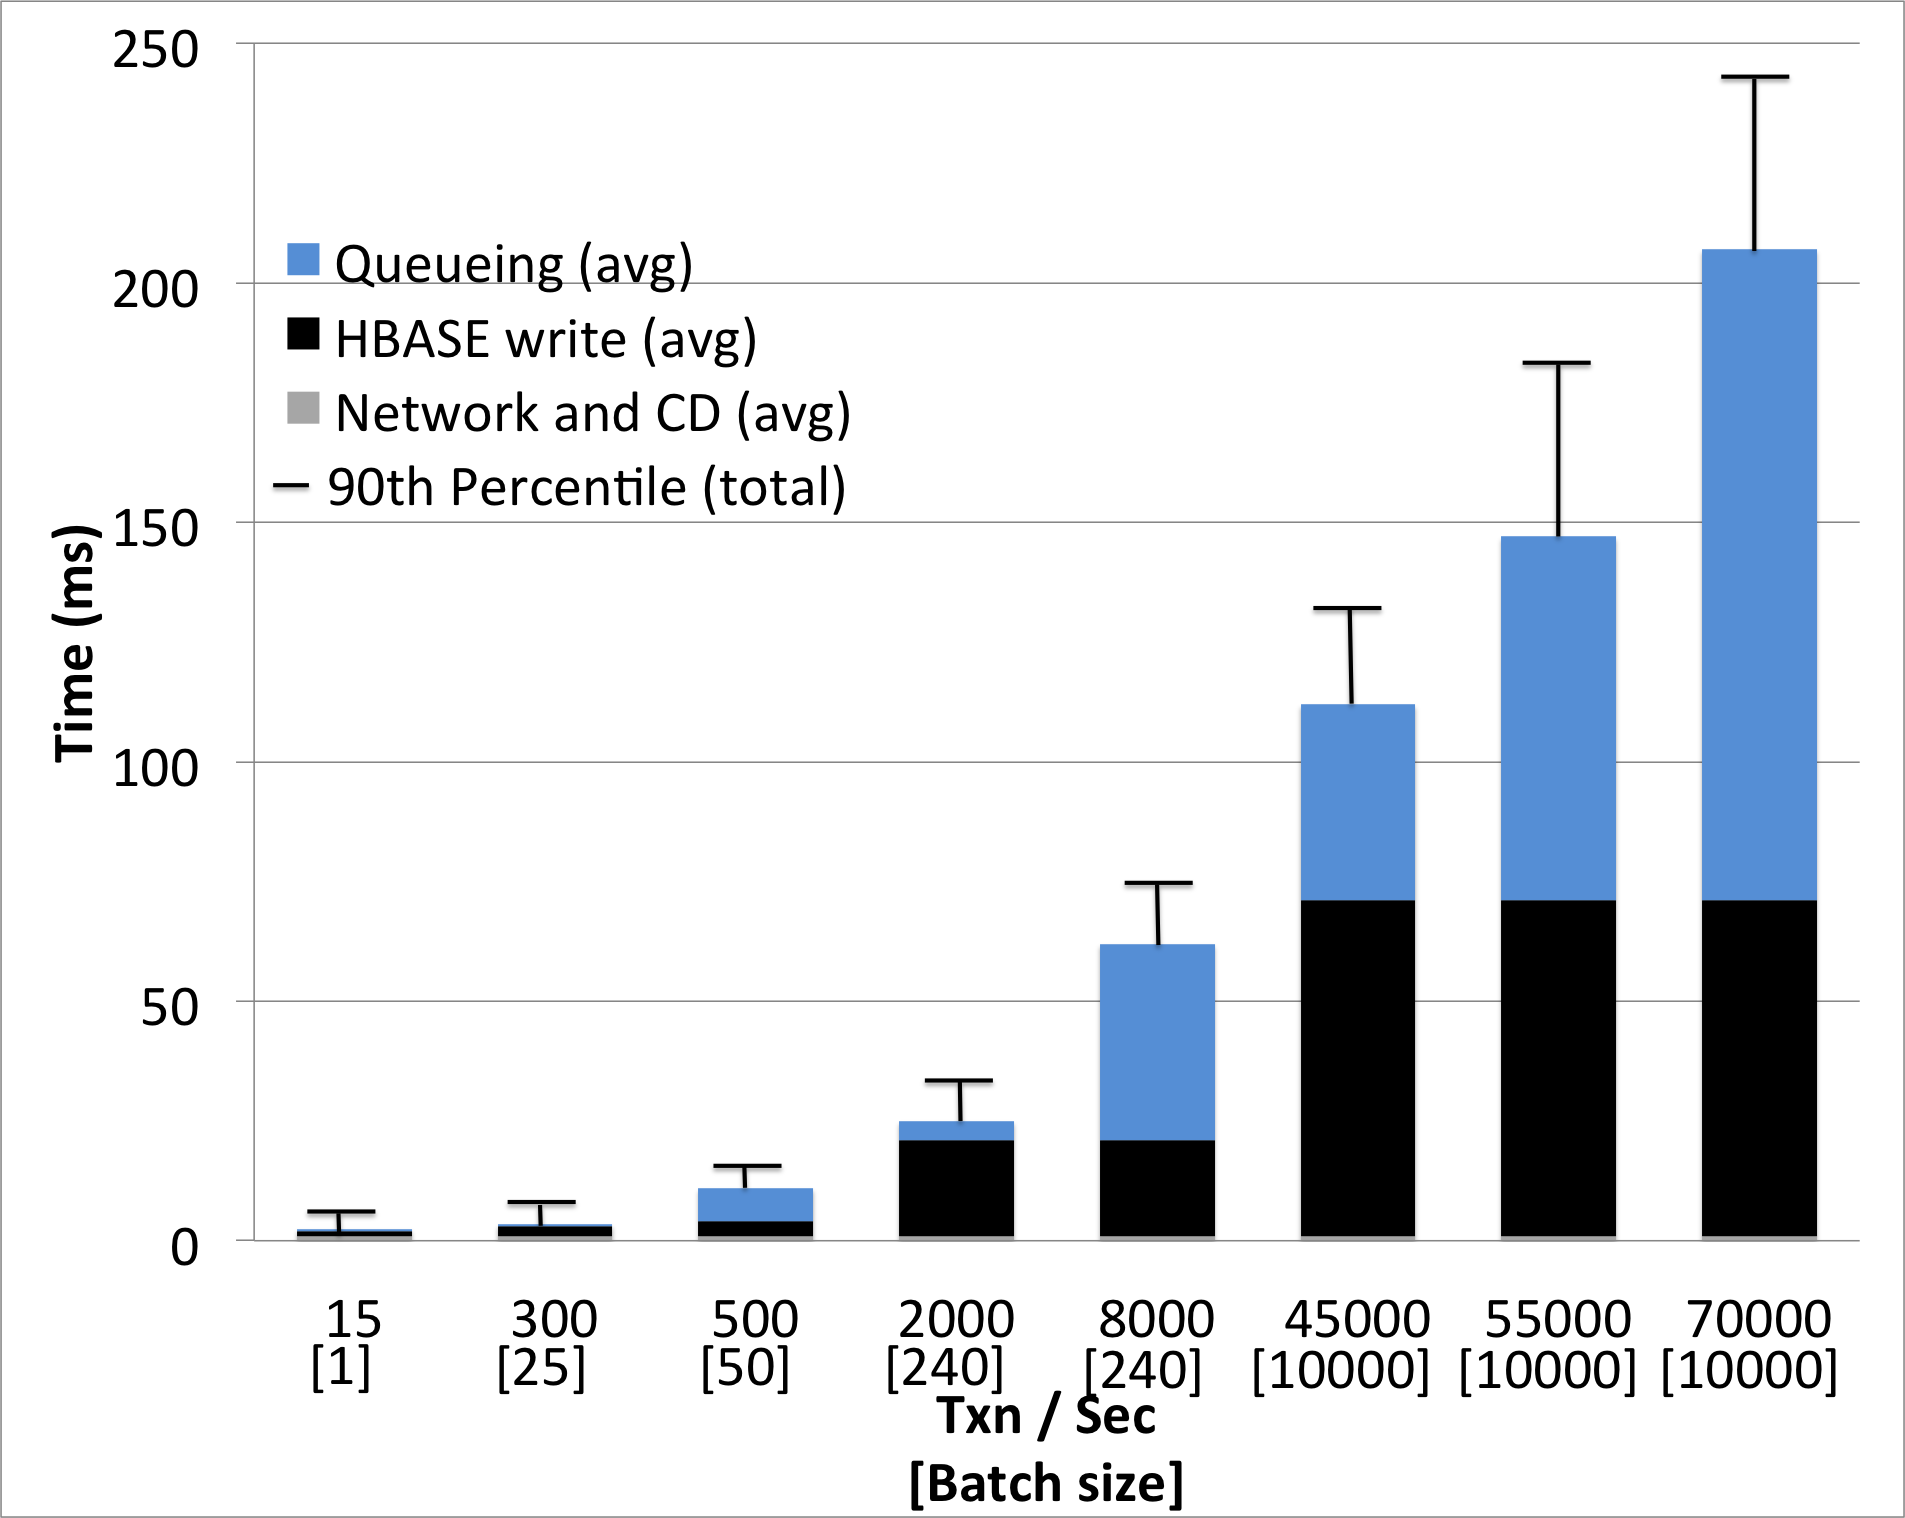
\includegraphics[width=0.975\columnwidth]{Latency-Omid.png}
}
\caption{{\bf \sys\ throughput vs.\ latency.} Client-perceived commit latency (average broken down and $90\%$ of total); single region server; power-law transaction sizes  with $\alpha=1.6$; batch sizes optimized for minimum latency (in square brackets below each bar).
}
\label{fig:omid_latency}
\end{figure}

\begin{figure}[h!]
\centerline{
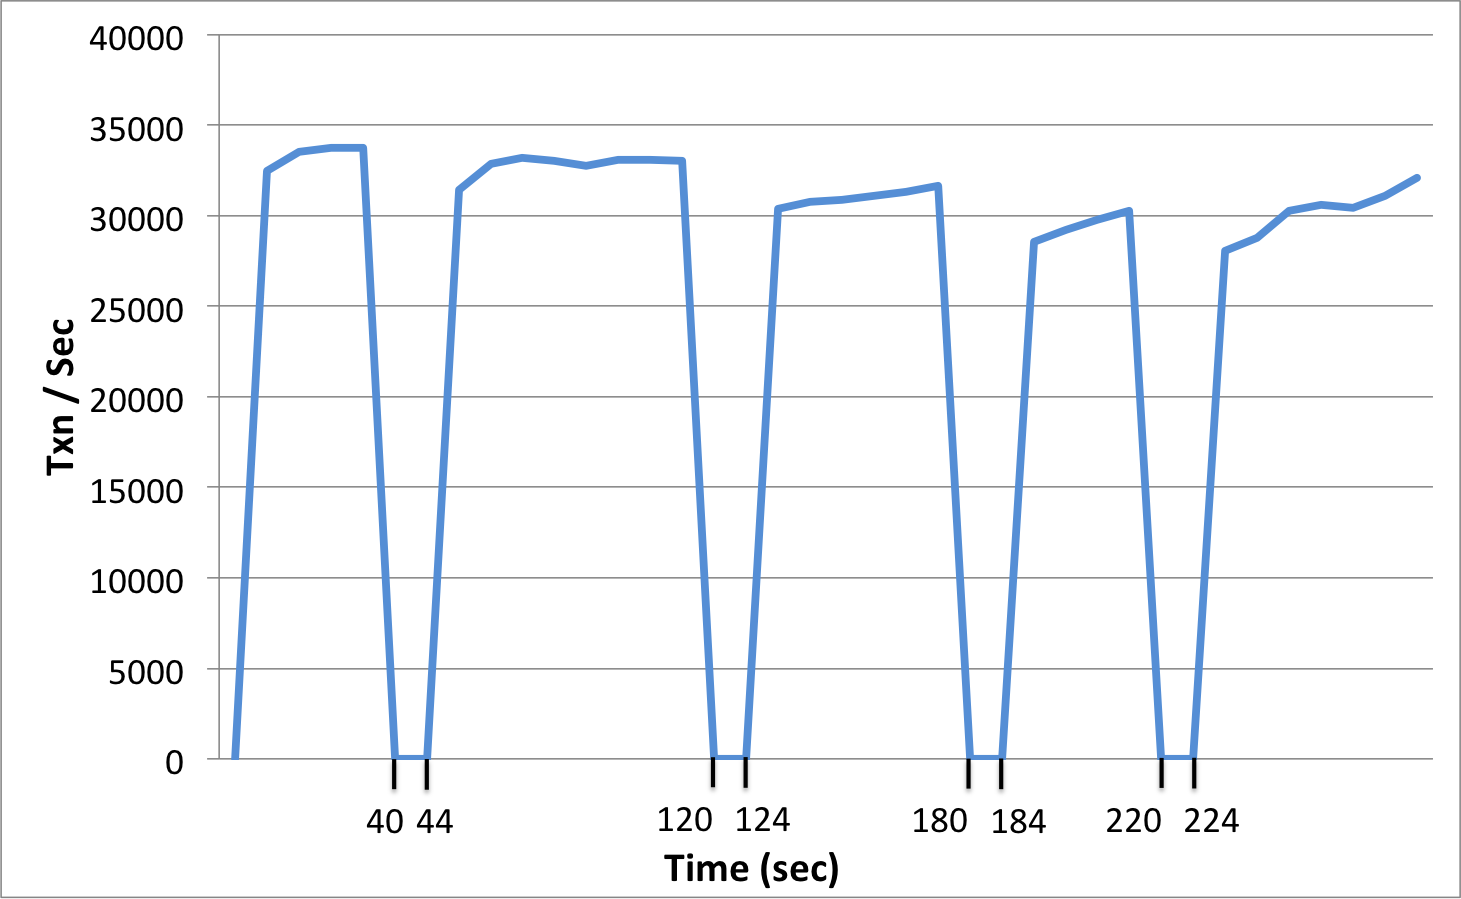
\includegraphics[width=\columnwidth]{HA.png}
}
\caption{{\bf \sys\ throughput with four failovers}; recovery takes around $4$ seconds. }
\label{fig:ha_recovery}
\end{figure}


\subsubsection{High availability}
\label{sec:ha-eval}


Finally, we exercise the high-availability mechanism. As long as the primary TM does not fail, HA induces negligible overhead. 
We now examine the system's recovery following a primary TM failure.  
The failure detection timeout is $\delta=1$ sec.
Figure~\ref{fig:ha_recovery} depicts  the system throughput over time, where the primary TM is forcefully shut down 
after  $40$ sec, is then allowed to recover, and the new primary (original backup) is shut down after $120$ sec. 
The primary is shut down two more times at $180$ and $220$ sec; the failover completes within $4$ sec.






\section{Lessons Learned and Future Work}
\label{sec:lessons}


\sys\ was originally designed as a foundational building block for Sieve -- Yahoo's next-generation content 
management platform. 
%Sieve ingests new content, and indexes it for search through a variety of processing steps in the real time. 
The need for transactions emerges in scenarios similar to Percolator~\cite{Percolator2010}.  
Analogously to other data pipelines, Sieve is more throughput-sensitive than latency-sensitive. This has led 
to a design that trades off latency for throughput via batching.
%, and scales the service on a single dedicated TM. 
The original design of Omid1~\cite{OmidICDE2014} did not employ a CT, but instead had the TM send clients information
about all pending transactions. This design was abandoned due to limited scalability in the number of clients,
 and was replaced by \sys, which uses the CT to track transaction states. The CT may be sharded for I/O scalability, 
but its update rate is bounded by the resources of the single (albeit multi-threaded) TM; this is mitigated by batching.
%which is a good fit for throughput-oriented applications like Sieve.

%Once \sys\ has been released to open source and became an Apache Incubator project, new use cases began to arise. 
Since becoming an Apache Incubator project, Omid is witnessing increased interest, in a variety of use cases. 
Together with Tephra, it is being considered for use by Apache Phoenix -- an emerging OLTP SQL engine over HBase 
storage~\cite{phoenix}. In that context, latency has increased importance. We are therefore developing a low-latency 
version of \sys\, that has clients update the CT instead of the TM, which eliminates the need for batching and allows 
throughput scaling without sacrificing latency. Similar approaches have been used in Percolator~\cite{Percolator2010}, 
Corfu~\cite{BalakrishnanMDPWW13}, and CockroachDB~\cite{cockroach}. We note, however, that such decentralization 
induces extra synchronization oerhead at commit time and  may increase aborts (in particular, reads may induce aborts); 
the original design may be preferable for throughput-oriented systems.

%A second example, also raised by HortonWorks, was deploying the TM on a non-dedicated machine. Whereas in Sieve each TM runs
%on a dedicated server, there are use cases where \sys\ is just one of many deployed applications, each handling low traffic. 
%This has led us to develop a less CPU-intensive  version of the TM (with no busy waiting for messages) for the open-source project.

Another development %driven by feedback from the open-source community 
is using application semantics to reduce conflict detection. Specifically, some applications can identify scenarios where conflicts 
need not be checked because the use case ensures that they won't happen. Consider, e.g., a massive table load, where records 
are inserted sequentially, hence no conflicts can arise. Another example is a secondary index update, which is guaranteed
to induce no conflict given that the primary table update by the same transaction has been successful. 
To reduce overhead in such cases, we plan to extend the write API to indicate which written keys need
to be tracked for conflict detection. 

%Finally, it may be useful to integrate \sys\ with other persistent multi-versioned key-value stores.%, or use 
%the system to provide ACID transactions along with high-level access abstractions, e.g., a relational database over HBase~\cite{phoenix}. 
On the scalability side, faster technologies may be considered to maintain \sys's commit metadata.  In particular, since \sys's commit table 
is usually written sequentially and infrequently read, it might be more efficient to use log-structured storage that is better optimized for the 
above scenario. Modern hardware (e.g., SSD storage, RDMA networks)  could bring further speedups. 





\subsection*{Acknowledgments}

We acknowledge the many contributions to Omid, as concept and code, since its early days. 
Our thanks go to Aran Bergman, Daniel Gomez Ferro, Yonatan Gottesman, Flavio Junqueira, Igor Katkov, Francis Christopher Liu, 
Ralph Rabbat, Benjamin (Ben) Reed, Kostas Tsioutsiouliklis, Maysam Yabandeh, and the Sieve team at Yahoo.  We also thank 
Dahlia Malkhi and the FAST reviewers for insightful comments.


%%%%%%%%%%%%%%%%%%%%%
%\clearpage
\small
{\bibliographystyle{acm}
\bibliography{refs}}

%%\theendnotes


\end{document}
